\documentclass[a4paper]{article}
\usepackage{aqis}
\usepackage{enumitem}
\usepackage{graphicx}
\usepackage{array}
\usepackage{booktabs}
% Indicator uses bold 1; no external dsfont package is required.
\usepackage{tikz}
\usetikzlibrary{calc,arrows.meta,decorations.markings}
\usepackage[colorlinks]{hyperref}
\usepackage{color}
\newcommand{\blue}[1]{\textcolor{blue}{#1}}

\newcommand{\rd}{r}
\newcommand{\gr}{g}
\newcommand{\bl}{b}
\newcommand{\pth}{p_{\mathrm{th}}}
\newcommand{\GF}{\mathrm{GF}(2)}
\providecommand{\ket}[1]{\ensuremath{|#1\rangle}}
\providecommand{\bra}[1]{\ensuremath{\langle#1|}}
% edges and triangles of the lattice (Sec. 2)
\newcommand{\eh}[1]{e^{\rightarrow}_{#1}}   % horizontal edge  (x,y)->(x+1,y)
\newcommand{\ev}[1]{e^{\uparrow}_{#1}}      % vertical edge    (x,y)->(x,y+1)
\newcommand{\ed}[1]{e^{\nearrow}_{#1}}      % diagonal edge    (x,y)->(x+1,y+1)
\newcommand{\tlo}[1]{\Delta^{\mathrm{lo}}_{#1}}
\newcommand{\tup}[1]{\Delta^{\mathrm{up}}_{#1}}

%% v11 (2026-11-10; v10: 2026-11-03): manuscript of study 1. History: v8 -> v9.1 (review of 2026-11-01: R1-1, R1-3, R1-7,
%% Gemini 1.3) -> v9.2 (holonomy restriction, CZ residual after flux removal, interpretation of the control
%% experiment, proof of the measurement update, measurement-circuit figure) -> v10 (labels only) -> v11 (labels only).
%% Numbers: production data of the v7 code (= v10 = v11 for code capacity and phenomenological noise), 10^4 shots per
%% point, L <= 9. Blue = to be replaced after the 10^5-shot production runs and the GPU validation of the
%% present circuit-level model. Build: pdflatex main_v11.tex (twice).
\begin{document}

\title{Non-Commuting Dressed Stabilizers and the $X$-Stabilizer Threshold\\ of the $\mathbb{D}_4$ Clifford-Hierarchy Code}

\author{
  Claude
}

\abstract{
The two-dimensional $\mathbb{D}_4$ Clifford-hierarchy stabilizer code of Kobayashi, Zhu, and Hsin supports transversal non-Clifford gates, but its $X$-type stabilizers are Pauli operators dressed by controlled-$Z$ (CZ) gates. Measuring them requires CCZ gates, and, more fundamentally, dressed stabilizers of different colors can stop commuting when an $X$ error creates a flux: corresponding outcomes can become random and depend on the order and timing of the measurements. A previous threshold estimate replaced the dressed measurement by commuting Pauli checks plus independent $Z$ noise and could therefore not represent this effect. We show that, under Pauli noise, the state of the code during arbitrary sequences of dressed measurements remains a uniform superposition over an affine space of flat gauge configurations, whose phase differs from the (cubic) phase of the initial code state by a quadratic form over $\GF$. This yields an exact sampler whose cost grows polynomially with the system size. It is a special case of the Clifford-stabilizer simulation of Takada, Bartlett and Williamson, and we verify it against brute-force state-vector simulation at $L=3$ and against an independent implementation of that method at $L\le9$. Combined with just-in-time correction of fluxes and matching decoders, it gives finite-size crossings of the $X$-stabilizer (charge-sector) failure rate of $9$--$10\%$ for code-capacity noise, $2.25\%$, $2.09\%$ and $2.00\%$ for $L=3$--$5$, $5$--$7$ and $7$--$9$ under phenomenological noise, and about $\blue{0.2\%}$ for circuit-level noise with native CCZ gates. Under phenomenological and circuit-level noise the crossings still drift to lower $p$ with $L$, so these are finite-size estimates, not asymptotic thresholds. A control experiment compares the complete dressed and undressed models; at circuit level this includes the additional gate faults, not only non-commutativity.
}

\keywords{Quantum Error Correction, Clifford-Hierarchy Stabilizer Codes, Non-Abelian Topological Order, Just-in-Time Decoding, Error Threshold, Classical Simulation}

\maketitle

%########### body

\section{Introduction}
\label{sec:intro}

Universal fault-tolerant quantum computation requires logical gates outside the Clifford group~\cite{eastin-knill2009}, and for topological Pauli stabilizer codes in $n$ dimensions the transversal (more generally, constant-depth) logical gates are confined to the $n$-th level of the Clifford hierarchy~\cite{bravyikonig2013}. Kobayashi, Zhu, and Hsin recently introduced \emph{Clifford-hierarchy stabilizer codes}, whose stabilizer groups contain non-Pauli operators and which evade this restriction~\cite{kobayashi2025clifford}. In two dimensions their construction gives a Clifford stabilizer code equivalent to a twisted $\mathbb{Z}_2^3$ gauge theory, i.e.\ to the non-Abelian $\mathbb{D}_4$ topological order that has been realized on a trapped-ion processor~\cite{iqbal2024nonabelian}, and it supports transversal logical $T$ and $CS$ gates. Closely related non-Abelian codes are at the heart of recent proposals for universal fault-tolerant computation in two dimensions~\cite{davydova2025knots,magdalena2026}.

The $Z$-type stabilizers of this code are ordinary Pauli plaquette operators, but its $X$-type stabilizers are vertex operators \emph{dressed} by CZ gates. Two difficulties follow. First, measuring a dressed stabilizer with an ancilla promotes each CZ to a CCZ gate, so the syndrome-extraction circuit is non-Clifford and cannot be sampled with stabilizer simulators such as Stim~\cite{gidney2021stim,gottesmanknill1998}; universal simulators such as Tsim~\cite{haenel2026tsim} scale exponentially with the number of non-Clifford gates. Second, and more fundamentally, the dressed stabilizers commute only in the flux-free subspace. Once an $X$ error has created a flux, dressed stabilizers of different colors can anticommute, and measuring one of them randomizes the other. The syndrome of the $X$-stabilizers is then no longer a deterministic function of an error configuration: it depends on which checks were measured, in which order, and for how long the flux survived.

A previous study~\cite{haga2026aqis} estimated the $X$-stabilizer thresholds of this code with a Clifford surrogate. The dressed checks were replaced by bare Pauli-$X$ checks, and the effect of the dressing was reinjected as independent $Z$ noise on the dressed qubit pairs at a rate $r=\kappa c p$, with $\kappa$ calibrated at distance $3$ against exact simulations of a single check measured twice. That study reported thresholds of $2.6\%$, $2.4\%$ and $0.62\%$ for three noise models. In this work we show that this construction misses the non-commutativity described above (Sec.~\ref{sec:noncomm}), explain why its calibration could not detect the discrepancy, and replace it by a simulation that treats the dressed measurements exactly. The noise models themselves have also been redefined; Sec.~\ref{sec:noise} states the old and new definitions side by side.

Our contributions are as follows. (i) We derive the commutator of two dressed stabilizers and show explicitly how an $X$ error turns a dressed measurement into a random one whose effect persists for the lifetime of the flux. (ii) We prove that, for Pauli noise and native CCZ gates, all states reached by the syndrome-extraction protocol are described by an affine subspace of the selected flat gauge configurations and a quadratic phase over $\GF$, which gives an exact and efficient sampler. (iii) We embed the sampler in a memory protocol in which fluxes are detected by the $Z$-plaquettes and removed in real time by a just-in-time (JIT) decoder, as required for this code~\cite{kobayashi2025clifford,davydova2025knots}; the previous study did not correct fluxes at all. (iv) We verify the sampler against an independent brute-force state-vector simulation at $L=3$ and, trajectory by trajectory, against an independent implementation of the Clifford-stabilizer (Pauli-proxy) simulation of Takada \emph{et al.}~\cite{takada2026exact} at $L=3,5,7,9$. (v) We report finite-size crossings of the $X$-stabilizer failure rate for three noise models and compare the chosen dressed and undressed models by a control experiment. This changes the code and, at circuit level, removes CCZ gates and their faults; it does not isolate non-commutativity alone.

To keep the paper self-contained, Sec.~\ref{sec:d4} sets up explicit lattice coordinates and evaluates the cup products of Ref.~\cite{kobayashi2025clifford} on our lattice, so that every stabilizer used later can be written down qubit by qubit; we use $L=3$ as a running example.

%=====================================================================
\section{The \texorpdfstring{$\mathbb{D}_4$}{D4} Code on a Triangulated Torus}
\label{sec:d4}

\paragraph{Lattice and coordinates.}
We use the code of Ref.~\cite{kobayashi2025clifford} on an $L\times L$ square lattice with periodic boundary conditions, in which every unit square is cut by a diagonal running from its lower-left to its upper-right corner (Fig.~\ref{fig:lattice}a). Vertices are labelled $(x,y)$ with $x,y\in\{0,1,\dots,L-1\}$, and all coordinates are understood modulo $L$; at $L=3$, for example, $(-1,0)\equiv(2,0)$ and $(0,3)\equiv(0,0)$. Each vertex $(x,y)$ is the starting point of three edges,
\begin{align}
  \eh{x,y}&=(x,y)\to(x+1,y), \nonumber\\
  \ev{x,y}&=(x,y)\to(x,y+1), \\
  \ed{x,y}&=(x,y)\to(x+1,y+1),\nonumber
\end{align}
so there are $3L^2$ edges. Each unit square with lower-left corner $(x,y)$ contains two triangles (plaquettes),
\begin{align}
  \tlo{x,y}&=\langle(x,y),(x+1,y),(x+1,y+1)\rangle,\nonumber\\
  \tup{x,y}&=\langle(x,y),(x,y+1),(x+1,y+1)\rangle,
  \label{eq:triangles}
\end{align}
below and above the diagonal, i.e.\ $2L^2$ triangles in total. The order in which we list the corners of a triangle defines its \emph{branching}, $\langle v_0,v_1,v_2\rangle$: $v_0$ is always the lower-left and $v_2$ the upper-right corner of the square. Every edge then points from its lower-order to its higher-order end, i.e.\ to the right, upwards, or diagonally upwards, and the two triangles that share an edge agree on its direction. In the notation $e_{ij}=(v_i\to v_j)$,
\begin{align}
  \tlo{x,y}&:\ e_{01}=\eh{x,y},\ e_{12}=\ev{x+1,y},\ e_{02}=\ed{x,y},\nonumber\\
  \tup{x,y}&:\ e_{01}=\ev{x,y},\ e_{12}=\eh{x,y+1},\ e_{02}=\ed{x,y}.
  \label{eq:triedges}
\end{align}
This is exactly the lattice built by our implementation.

\paragraph{Qubits and gauge configurations.}
Each edge $e$ carries three qubits, labelled by a color $c\in\{\rd,\gr,\bl\}$; the colors simply distinguish three copies of a $\mathbb{Z}_2$ gauge field. Hence $n=9L^2$ (81 at $L=3$). We write $X^c_e$, $Z^c_e$ for the Pauli operators on qubit $(e,c)$. A computational-basis state is labelled by a bit string $a\in\GF^{n}$, with
\begin{equation}
  Z^c_e\ket{a}=(-1)^{a_c(e)}\ket{a},\qquad X^c_e\ket{a}=\ket{a+\mathbf 1_{(e,c)}},
  \label{eq:basis}
\end{equation}
where $\mathbf 1_{(e,c)}$ is the unit vector of qubit $(e,c)$ and addition is modulo 2. For a fixed color, $a_c$ assigns a bit to every edge; in the language of Ref.~\cite{kobayashi2025clifford} it is a $\mathbb{Z}_2$ \emph{1-cochain}, and the triple $a=(a_\rd,a_\gr,a_\bl)$ is a \emph{gauge configuration}. For any $s\in\GF^n$ we write $X^s=\prod_{q:\,s_q=1}X_q$, so that $X^s\ket{a}=\ket{a+s}$.

\paragraph{$Z$-stabilizers and fluxes.}
For a triangle $\Delta=\langle v_0,v_1,v_2\rangle$ let $(da_c)(\Delta)=a_c(e_{01})+a_c(e_{12})+a_c(e_{02})\bmod 2$. The $Z$-stabilizers are the $3\times2L^2$ plaquette operators
\begin{equation}
  S^{c}_{Z;\Delta}=\prod_{e\in\partial \Delta}Z^{c}_e=(-1)^{(da_c)(\Delta)},
  \label{eq:zstab}
\end{equation}
e.g.\ $S^\rd_{Z;\tlo{0,0}}=Z^\rd_{\eh{0,0}}Z^\rd_{\ev{1,0}}Z^\rd_{\ed{0,0}}$. A configuration is \emph{flat} if $da_c=0$ for all colors and all triangles, and a triangle with $(da_c)(\Delta)=1$ is called a flux of color $c$. A single error $X^c_e$ flips $a_c(e)$ and therefore creates fluxes of color $c$ on the two triangles that contain $e$; for example, $X^\gr_{\eh{0,0}}$ creates green fluxes on $\tlo{0,0}$ and $\tup{0,-1}$.

\paragraph{Cup products on this lattice.}
Ref.~\cite{kobayashi2025clifford} specifies the dressing of the $X$-stabilizers through cup products. On a triangle with branching $\langle v_0,v_1,v_2\rangle$, the cup product of a 0-cochain $\alpha$ (a function on vertices) with two 1-cochains $\beta,\gamma$ is evaluated as~\cite{kobayashi2025clifford}
\begin{align}
  (\alpha\cup\beta\cup\gamma)(\Delta)&=\alpha(v_0)\,\beta(e_{01})\,\gamma(e_{12}),\nonumber\\
  (\beta\cup\alpha\cup\gamma)(\Delta)&=\beta(e_{01})\,\alpha(v_1)\,\gamma(e_{12}),\label{eq:cup}\\
  (\beta\cup\gamma\cup\alpha)(\Delta)&=\beta(e_{01})\,\gamma(e_{12})\,\alpha(v_2),\nonumber
\end{align}
and $\int\omega=\sum_\Delta\sigma(\Delta)\,\omega(\Delta)$, where $\sigma(\Delta)=\pm1$ is the orientation induced by the branching. Since we only need these integrals modulo 2, the signs $\sigma$ drop out and $\int\omega=\sum_\Delta\omega(\Delta)\bmod 2$. Let $\tilde v$ be the indicator 0-cochain of the vertex $v=(x,y)$. The only triangles with $v_0=v$ are $\tlo{x,y}$ and $\tup{x,y}$, so Eqs.~\eqref{eq:triedges} and \eqref{eq:cup} give
\begin{equation}
  \int\tilde v\cup a_\gr\cup a_\bl
  =a_\gr(\eh{x,y})\,a_\bl(\ev{x+1,y})+a_\gr(\ev{x,y})\,a_\bl(\eh{x,y+1}).
  \label{eq:cupR}
\end{equation}
Likewise, $v=v_1$ for $\tlo{x-1,y}$ and $\tup{x,y-1}$, and $v=v_2$ for $\tlo{x-1,y-1}$ and $\tup{x-1,y-1}$, which gives
\begin{align}
  \int a_\rd\cup\tilde v\cup a_\bl
  &=a_\rd(\eh{x-1,y})\,a_\bl(\ev{x,y})+a_\rd(\ev{x,y-1})\,a_\bl(\eh{x,y}),\nonumber\\
  \int a_\rd\cup a_\gr\cup\tilde v
  &=a_\rd(\eh{x-1,y-1})\,a_\gr(\ev{x,y-1})\nonumber\\
  &\quad+a_\rd(\ev{x-1,y-1})\,a_\gr(\eh{x-1,y}).
  \label{eq:cupGB}
\end{align}

\paragraph{From CZ gates to a phase $(-1)^{q(a)}$.}
A CZ gate is diagonal in the computational basis: by definition $\mathrm{CZ}=\mathrm{diag}(1,1,1,-1)$, i.e.
\begin{equation}
  \mathrm{CZ}_{i,j}\ket{a}=(-1)^{a_ia_j}\ket{a}.
  \label{eq:cz}
\end{equation}
This is an exact identity, not an approximation. Diagonal operators commute with each other and their phases add, so for any set $P$ of qubit pairs $\prod_{(i,j)\in P}\mathrm{CZ}_{i,j}\ket{a}=(-1)^{\sum_{(i,j)\in P}a_ia_j}\ket{a}$, independently of the order of the gates. Ref.~\cite{kobayashi2025clifford} writes the dressing of $S^\rd_{X;v}$ as a product of $\mathrm{CZ}^{\gr,\bl}_{e',e''}$ over all edge pairs with $\int\tilde v\cup\tilde e'\cup\tilde e''\neq0$. By Eq.~\eqref{eq:cup} these are exactly the pairs $(e_{01},e_{12})$ of the triangles with $v_0=v$, and since $a_\gr=\sum_{e'}a_\gr(e')\,\tilde e'$ and the cup product is bilinear,
\begin{equation}
  \prod_{e',e'':\,\int\tilde v\cup\tilde e'\cup\tilde e''\neq0}\mathrm{CZ}^{\gr,\bl}_{e',e''}
  =(-1)^{\int\tilde v\cup a_\gr\cup a_\bl}
  \label{eq:czcup}
\end{equation}
as an operator identity. The same holds for the other two colors.

\paragraph{$X$-stabilizers in coordinates.}
For every vertex $v=(x,y)$ and color $c$ there is one $X$-stabilizer~\cite{kobayashi2025clifford},
\begin{equation}
  S^{\rd}_{X;v}=\Big(\prod_{e\ni v}X^{\rd}_e\Big)\,(-1)^{\int \tilde v\cup a_\gr\cup a_\bl},
  \label{eq:xstab}
\end{equation}
and similarly $S^{\gr}_{X;v}$ and $S^{\bl}_{X;v}$ with phases $(-1)^{\int a_\rd\cup\tilde v\cup a_\bl}$ and $(-1)^{\int a_\rd\cup a_\gr\cup\tilde v}$. The product runs over the six edges that end at $v$,
\begin{equation}
  e\ni v:\quad \eh{x,y},\ \eh{x-1,y},\ \ev{x,y},\ \ev{x,y-1},\ \ed{x,y},\ \ed{x-1,y-1}.
  \label{eq:star}
\end{equation}
By Eqs.~\eqref{eq:cupR}--\eqref{eq:czcup}, the dressing consists of two CZ gates per check:
\begin{align}
  S^\rd_{X;v}&:\ \mathrm{CZ}\big(\gr\,\eh{x,y},\,\bl\,\ev{x+1,y}\big)\,\mathrm{CZ}\big(\gr\,\ev{x,y},\,\bl\,\eh{x,y+1}\big),\nonumber\\
  S^\gr_{X;v}&:\ \mathrm{CZ}\big(\rd\,\eh{x-1,y},\,\bl\,\ev{x,y}\big)\,\mathrm{CZ}\big(\rd\,\ev{x,y-1},\,\bl\,\eh{x,y}\big),\label{eq:czlist}\\
  S^\bl_{X;v}&:\ \mathrm{CZ}\big(\rd\,\eh{x-1,y-1},\,\gr\,\ev{x,y-1}\big)\,\mathrm{CZ}\big(\rd\,\ev{x-1,y-1},\,\gr\,\eh{x-1,y}\big),\nonumber
\end{align}
where $\mathrm{CZ}(c\,e,c'\,e')$ acts on qubits $(e,c)$ and $(e',c')$ (Fig.~\ref{fig:lattice}b--d). So each check contains six Pauli-$X$ operators and two CZ gates. Qubits on diagonal edges never appear in a CZ gate, every other qubit appears in exactly two, and there are $6L^2$ CZ gates in total.

\begin{figure*}[t]
\centering
% fig_lattice.tex -- drawing of Figure 1 of main_v8.tex (lattice, coordinates, X-stabilizers).
% Included inside the figure* environment of main_v8.tex via % fig_lattice.tex -- drawing of Figure 1 of main_v8.tex (lattice, coordinates, X-stabilizers).
% Included inside the figure* environment of main_v8.tex via % fig_lattice.tex -- drawing of Figure 1 of main_v8.tex (lattice, coordinates, X-stabilizers).
% Included inside the figure* environment of main_v8.tex via \input{fig_lattice}.
% Needs from the preamble of main_v8.tex: \usepackage{tikz},
%   \usetikzlibrary{calc,arrows.meta,decorations.markings}, and the macros
%   \eh, \ev, \ed, \tlo, \tup, \rd, \gr, \bl.
% colors for the figures
\definecolor{cR}{rgb}{0.80,0.10,0.10}
\definecolor{cG}{rgb}{0.05,0.55,0.15}
\definecolor{cB}{rgb}{0.10,0.25,0.85}

% ---------- helper macros for the drawings ----------
\tikzset{
  edge/.style={gray!55,line width=0.5pt,
     postaction={decorate,decoration={markings,mark=at position 0.62 with {\arrow{Stealth[length=3pt]}}}}},
  xedge/.style={line width=1.6pt},
  qb/.style={circle,inner sep=0pt,minimum size=2.6pt,fill=gray!45},
  qx/.style={circle,inner sep=0pt,minimum size=4.6pt,draw=white,line width=0.4pt},
  czl/.style={densely dashed,line width=0.8pt,black},
  tri/.style={fill=yellow!35,draw=none},
}
% qubit positions along an edge P->Q: r at 0.28, g at 0.50, b at 0.72
\newcommand{\Qp}[5]{($(#1,#2)!#5!(#3,#4)$)}
\begin{tikzpicture}[scale=1.05,font=\scriptsize]
  % ================= (a) L=3 torus =================
  \begin{scope}
    \node[font=\small\bfseries] at (-0.55,3.45) {(a)};
    % triangles of square (0,0)
    \fill[yellow!25] (0,0)--(1,0)--(1,1)--cycle;
    \fill[orange!18] (0,0)--(0,1)--(1,1)--cycle;
    \node[font=\tiny,fill=white,fill opacity=0.7,text opacity=1,inner sep=0.5pt] at (0.63,0.36) {$\tlo{0,0}$};
    \node[font=\tiny,fill=white,fill opacity=0.7,text opacity=1,inner sep=0.5pt] at (0.40,0.64) {$\tup{0,0}$};
    \foreach \x in {0,1,2} \foreach \y in {0,1,2} {
      \draw[edge] (\x,\y)--(\x+1,\y);
      \draw[edge] (\x,\y)--(\x,\y+1);
      \draw[edge] (\x,\y)--(\x+1,\y+1);
    }
    % periodic copies
    \draw[gray!40,dashed] (0,3)--(3,3)--(3,0);
    % support of S^r_X at (0,0) and its periodic images
    \foreach \xa/\ya/\xb/\yb in {0/0/1/0, 2/0/3/0, 0/0/0/1, 0/2/0/3, 0/0/1/1, 2/2/3/3}{
      \draw[cR,xedge,opacity=0.35] (\xa,\ya)--(\xb,\yb);
      \node[qx,fill=cR] at \Qp{\xa}{\ya}{\xb}{\yb}{0.28} {};
    }
    % CZ pairs of S^r_X at (0,0)
    \node[qx,fill=cG] (g1) at \Qp{0}{0}{1}{0}{0.5} {};
    \node[qx,fill=cB] (b1) at \Qp{1}{0}{1}{1}{0.72} {};
    \node[qx,fill=cG] (g2) at \Qp{0}{0}{0}{1}{0.5} {};
    \node[qx,fill=cB] (b2) at \Qp{0}{1}{1}{1}{0.72} {};
    \draw[czl] (g1) to[bend right=25] (b1);
    \draw[czl] (g2) to[bend left=25] (b2);
    % vertices
    \foreach \x in {0,1,2,3} \foreach \y in {0,1,2,3} {
      \fill (\x,\y) circle (1.1pt);
    }
    \foreach \x in {0,1,2} \node[below=1pt,font=\tiny] at (\x,0) {$x{=}\x$};
    \foreach \y in {0,1,2} \node[left=1pt,font=\tiny] at (0,\y) {$y{=}\y$};
    \node[below=1pt,font=\tiny,gray] at (3,0) {$x{=}3{\equiv}0$};
    \node[left=1pt,font=\tiny,gray] at (0,3) {$y{=}3{\equiv}0$};
    % edge labels of square (1,1)
    \node[anchor=north,font=\tiny,inner sep=1pt] at (1.5,0.98) {$\eh{1,1}$};
    \node[anchor=east,font=\tiny,inner sep=1pt] at (0.98,1.5) {$\ev{1,1}$};
    \node[anchor=south east,font=\tiny,inner sep=0.5pt] at (1.45,1.58) {$\ed{1,1}$};
    % three qubits per edge (legend)
    \begin{scope}[shift={(0.2,-1.05)}]
      \draw[gray!55,line width=0.5pt] (0,0)--(1.6,0);
      \node[qx,fill=cR] at (0.448,0) {}; \node[qx,fill=cG] at (0.8,0) {}; \node[qx,fill=cB] at (1.152,0) {};
      \node[anchor=west,align=left,font=\tiny] at (1.7,0) {three qubits $(e,\rd),(e,\gr),(e,\bl)$ on every edge $e$};
    \end{scope}
  \end{scope}
  % ================= (b)-(d) local pictures =================
  \foreach \col/\name/\lab/\px in {cR/\rd/(b)/5.0, cG/\gr/(c)/8.0, cB/\bl/(d)/11.0} {
    \begin{scope}[shift={(\px,1.5)}]
      \node[font=\small\bfseries] at (-1.45,1.95) {\lab};
      \node[font=\small] at (0.25,1.95) {$S^{\name}_{X;(x,y)}$};
    \end{scope}
  }
  % ---- (b) red ----
  \begin{scope}[shift={(5.0,1.5)}]
    \fill[yellow!35] (0,0)--(1,0)--(1,1)--cycle; \fill[orange!18] (0,0)--(0,1)--(1,1)--cycle;
    \foreach \x in {-1,0} \foreach \y in {-1,0} {
      \draw[edge] (\x,\y)--(\x+1,\y); \draw[edge] (\x,\y)--(\x,\y+1); \draw[edge] (\x,\y)--(\x+1,\y+1);}
    \draw[edge] (-1,1)--(0,1); \draw[edge] (0,1)--(1,1); \draw[edge] (1,-1)--(1,0); \draw[edge] (1,0)--(1,1);
    \foreach \xa/\ya/\xb/\yb in {0/0/1/0, -1/0/0/0, 0/0/0/1, 0/-1/0/0, 0/0/1/1, -1/-1/0/0}{
      \draw[cR,xedge,opacity=0.35] (\xa,\ya)--(\xb,\yb); \node[qx,fill=cR] at \Qp{\xa}{\ya}{\xb}{\yb}{0.28} {};}
    \node[qx,fill=cG] (a1) at \Qp{0}{0}{1}{0}{0.5} {}; \node[qx,fill=cB] (a2) at \Qp{1}{0}{1}{1}{0.72} {};
    \node[qx,fill=cG] (a3) at \Qp{0}{0}{0}{1}{0.5} {}; \node[qx,fill=cB] (a4) at \Qp{0}{1}{1}{1}{0.72} {};
    \draw[czl] (a1) to[bend right=25] (a2); \draw[czl] (a3) to[bend left=25] (a4);
    \foreach \x in {-1,0,1} \foreach \y in {-1,0,1} \fill (\x,\y) circle (1.1pt);
    \node[anchor=north east,inner sep=1pt,font=\tiny] at (0,0) {$v{=}v_0$};
  \end{scope}
  % ---- (c) green ----
  \begin{scope}[shift={(8.0,1.5)}]
    \fill[yellow!35] (-1,0)--(0,0)--(0,1)--cycle; \fill[orange!18] (0,-1)--(0,0)--(1,0)--cycle;
    \foreach \x in {-1,0} \foreach \y in {-1,0} {
      \draw[edge] (\x,\y)--(\x+1,\y); \draw[edge] (\x,\y)--(\x,\y+1); \draw[edge] (\x,\y)--(\x+1,\y+1);}
    \draw[edge] (-1,1)--(0,1); \draw[edge] (0,1)--(1,1); \draw[edge] (1,-1)--(1,0); \draw[edge] (1,0)--(1,1);
    \foreach \xa/\ya/\xb/\yb in {0/0/1/0, -1/0/0/0, 0/0/0/1, 0/-1/0/0, 0/0/1/1, -1/-1/0/0}{
      \draw[cG,xedge,opacity=0.35] (\xa,\ya)--(\xb,\yb); \node[qx,fill=cG] at \Qp{\xa}{\ya}{\xb}{\yb}{0.5} {};}
    \node[qx,fill=cR] (a1) at \Qp{-1}{0}{0}{0}{0.28} {}; \node[qx,fill=cB] (a2) at \Qp{0}{0}{0}{1}{0.72} {};
    \node[qx,fill=cR] (a3) at \Qp{0}{-1}{0}{0}{0.28} {}; \node[qx,fill=cB] (a4) at \Qp{0}{0}{1}{0}{0.72} {};
    \draw[czl] (a1) to[bend left=30] (a2); \draw[czl] (a3) to[bend right=30] (a4);
    \foreach \x in {-1,0,1} \foreach \y in {-1,0,1} \fill (\x,\y) circle (1.1pt);
    \node[anchor=north west,inner sep=1pt,font=\tiny] at (0,0) {$v{=}v_1$};
  \end{scope}
  % ---- (d) blue ----
  \begin{scope}[shift={(11.0,1.5)}]
    \fill[yellow!35] (-1,-1)--(0,-1)--(0,0)--cycle; \fill[orange!18] (-1,-1)--(-1,0)--(0,0)--cycle;
    \foreach \x in {-1,0} \foreach \y in {-1,0} {
      \draw[edge] (\x,\y)--(\x+1,\y); \draw[edge] (\x,\y)--(\x,\y+1); \draw[edge] (\x,\y)--(\x+1,\y+1);}
    \draw[edge] (-1,1)--(0,1); \draw[edge] (0,1)--(1,1); \draw[edge] (1,-1)--(1,0); \draw[edge] (1,0)--(1,1);
    \foreach \xa/\ya/\xb/\yb in {0/0/1/0, -1/0/0/0, 0/0/0/1, 0/-1/0/0, 0/0/1/1, -1/-1/0/0}{
      \draw[cB,xedge,opacity=0.35] (\xa,\ya)--(\xb,\yb); \node[qx,fill=cB] at \Qp{\xa}{\ya}{\xb}{\yb}{0.72} {};}
    \node[qx,fill=cR] (a1) at \Qp{-1}{-1}{0}{-1}{0.28} {}; \node[qx,fill=cG] (a2) at \Qp{0}{-1}{0}{0}{0.5} {};
    \node[qx,fill=cR] (a3) at \Qp{-1}{-1}{-1}{0}{0.28} {}; \node[qx,fill=cG] (a4) at \Qp{-1}{0}{0}{0}{0.5} {};
    \draw[czl] (a1) to[bend right=30] (a2); \draw[czl] (a3) to[bend left=30] (a4);
    \foreach \x in {-1,0,1} \foreach \y in {-1,0,1} \fill (\x,\y) circle (1.1pt);
    \node[anchor=south west,inner sep=1pt,font=\tiny] at (0,0) {$v{=}v_2$};
  \end{scope}
  % legend for (b)-(d)
  \begin{scope}[shift={(5.6,-0.1)}]
    \draw[cR,xedge,opacity=0.35] (0,0)--(0.4,0); \node[qx,fill=cR] at (0.2,0) {};
    \node[anchor=west,font=\tiny] at (0.5,0) {Pauli $X$ on the qubit of the check's own color};
    \draw[czl] (0,-0.32)--(0.4,-0.32);
    \node[anchor=west,font=\tiny] at (0.5,-0.32) {CZ between two qubits of the other two colors};
    \fill[yellow!35] (0,-0.76) rectangle (0.2,-0.52); \fill[orange!18] (0.2,-0.76) rectangle (0.4,-0.52);
    \node[anchor=west,font=\tiny] at (0.5,-0.64) {triangles $\tlo{}$ / $\tup{}$ on which the cup product is evaluated};
  \end{scope}
\end{tikzpicture}
.
% Needs from the preamble of main_v8.tex: \usepackage{tikz},
%   \usetikzlibrary{calc,arrows.meta,decorations.markings}, and the macros
%   \eh, \ev, \ed, \tlo, \tup, \rd, \gr, \bl.
% colors for the figures
\definecolor{cR}{rgb}{0.80,0.10,0.10}
\definecolor{cG}{rgb}{0.05,0.55,0.15}
\definecolor{cB}{rgb}{0.10,0.25,0.85}

% ---------- helper macros for the drawings ----------
\tikzset{
  edge/.style={gray!55,line width=0.5pt,
     postaction={decorate,decoration={markings,mark=at position 0.62 with {\arrow{Stealth[length=3pt]}}}}},
  xedge/.style={line width=1.6pt},
  qb/.style={circle,inner sep=0pt,minimum size=2.6pt,fill=gray!45},
  qx/.style={circle,inner sep=0pt,minimum size=4.6pt,draw=white,line width=0.4pt},
  czl/.style={densely dashed,line width=0.8pt,black},
  tri/.style={fill=yellow!35,draw=none},
}
% qubit positions along an edge P->Q: r at 0.28, g at 0.50, b at 0.72
\newcommand{\Qp}[5]{($(#1,#2)!#5!(#3,#4)$)}
\begin{tikzpicture}[scale=1.05,font=\scriptsize]
  % ================= (a) L=3 torus =================
  \begin{scope}
    \node[font=\small\bfseries] at (-0.55,3.45) {(a)};
    % triangles of square (0,0)
    \fill[yellow!25] (0,0)--(1,0)--(1,1)--cycle;
    \fill[orange!18] (0,0)--(0,1)--(1,1)--cycle;
    \node[font=\tiny,fill=white,fill opacity=0.7,text opacity=1,inner sep=0.5pt] at (0.63,0.36) {$\tlo{0,0}$};
    \node[font=\tiny,fill=white,fill opacity=0.7,text opacity=1,inner sep=0.5pt] at (0.40,0.64) {$\tup{0,0}$};
    \foreach \x in {0,1,2} \foreach \y in {0,1,2} {
      \draw[edge] (\x,\y)--(\x+1,\y);
      \draw[edge] (\x,\y)--(\x,\y+1);
      \draw[edge] (\x,\y)--(\x+1,\y+1);
    }
    % periodic copies
    \draw[gray!40,dashed] (0,3)--(3,3)--(3,0);
    % support of S^r_X at (0,0) and its periodic images
    \foreach \xa/\ya/\xb/\yb in {0/0/1/0, 2/0/3/0, 0/0/0/1, 0/2/0/3, 0/0/1/1, 2/2/3/3}{
      \draw[cR,xedge,opacity=0.35] (\xa,\ya)--(\xb,\yb);
      \node[qx,fill=cR] at \Qp{\xa}{\ya}{\xb}{\yb}{0.28} {};
    }
    % CZ pairs of S^r_X at (0,0)
    \node[qx,fill=cG] (g1) at \Qp{0}{0}{1}{0}{0.5} {};
    \node[qx,fill=cB] (b1) at \Qp{1}{0}{1}{1}{0.72} {};
    \node[qx,fill=cG] (g2) at \Qp{0}{0}{0}{1}{0.5} {};
    \node[qx,fill=cB] (b2) at \Qp{0}{1}{1}{1}{0.72} {};
    \draw[czl] (g1) to[bend right=25] (b1);
    \draw[czl] (g2) to[bend left=25] (b2);
    % vertices
    \foreach \x in {0,1,2,3} \foreach \y in {0,1,2,3} {
      \fill (\x,\y) circle (1.1pt);
    }
    \foreach \x in {0,1,2} \node[below=1pt,font=\tiny] at (\x,0) {$x{=}\x$};
    \foreach \y in {0,1,2} \node[left=1pt,font=\tiny] at (0,\y) {$y{=}\y$};
    \node[below=1pt,font=\tiny,gray] at (3,0) {$x{=}3{\equiv}0$};
    \node[left=1pt,font=\tiny,gray] at (0,3) {$y{=}3{\equiv}0$};
    % edge labels of square (1,1)
    \node[anchor=north,font=\tiny,inner sep=1pt] at (1.5,0.98) {$\eh{1,1}$};
    \node[anchor=east,font=\tiny,inner sep=1pt] at (0.98,1.5) {$\ev{1,1}$};
    \node[anchor=south east,font=\tiny,inner sep=0.5pt] at (1.45,1.58) {$\ed{1,1}$};
    % three qubits per edge (legend)
    \begin{scope}[shift={(0.2,-1.05)}]
      \draw[gray!55,line width=0.5pt] (0,0)--(1.6,0);
      \node[qx,fill=cR] at (0.448,0) {}; \node[qx,fill=cG] at (0.8,0) {}; \node[qx,fill=cB] at (1.152,0) {};
      \node[anchor=west,align=left,font=\tiny] at (1.7,0) {three qubits $(e,\rd),(e,\gr),(e,\bl)$ on every edge $e$};
    \end{scope}
  \end{scope}
  % ================= (b)-(d) local pictures =================
  \foreach \col/\name/\lab/\px in {cR/\rd/(b)/5.0, cG/\gr/(c)/8.0, cB/\bl/(d)/11.0} {
    \begin{scope}[shift={(\px,1.5)}]
      \node[font=\small\bfseries] at (-1.45,1.95) {\lab};
      \node[font=\small] at (0.25,1.95) {$S^{\name}_{X;(x,y)}$};
    \end{scope}
  }
  % ---- (b) red ----
  \begin{scope}[shift={(5.0,1.5)}]
    \fill[yellow!35] (0,0)--(1,0)--(1,1)--cycle; \fill[orange!18] (0,0)--(0,1)--(1,1)--cycle;
    \foreach \x in {-1,0} \foreach \y in {-1,0} {
      \draw[edge] (\x,\y)--(\x+1,\y); \draw[edge] (\x,\y)--(\x,\y+1); \draw[edge] (\x,\y)--(\x+1,\y+1);}
    \draw[edge] (-1,1)--(0,1); \draw[edge] (0,1)--(1,1); \draw[edge] (1,-1)--(1,0); \draw[edge] (1,0)--(1,1);
    \foreach \xa/\ya/\xb/\yb in {0/0/1/0, -1/0/0/0, 0/0/0/1, 0/-1/0/0, 0/0/1/1, -1/-1/0/0}{
      \draw[cR,xedge,opacity=0.35] (\xa,\ya)--(\xb,\yb); \node[qx,fill=cR] at \Qp{\xa}{\ya}{\xb}{\yb}{0.28} {};}
    \node[qx,fill=cG] (a1) at \Qp{0}{0}{1}{0}{0.5} {}; \node[qx,fill=cB] (a2) at \Qp{1}{0}{1}{1}{0.72} {};
    \node[qx,fill=cG] (a3) at \Qp{0}{0}{0}{1}{0.5} {}; \node[qx,fill=cB] (a4) at \Qp{0}{1}{1}{1}{0.72} {};
    \draw[czl] (a1) to[bend right=25] (a2); \draw[czl] (a3) to[bend left=25] (a4);
    \foreach \x in {-1,0,1} \foreach \y in {-1,0,1} \fill (\x,\y) circle (1.1pt);
    \node[anchor=north east,inner sep=1pt,font=\tiny] at (0,0) {$v{=}v_0$};
  \end{scope}
  % ---- (c) green ----
  \begin{scope}[shift={(8.0,1.5)}]
    \fill[yellow!35] (-1,0)--(0,0)--(0,1)--cycle; \fill[orange!18] (0,-1)--(0,0)--(1,0)--cycle;
    \foreach \x in {-1,0} \foreach \y in {-1,0} {
      \draw[edge] (\x,\y)--(\x+1,\y); \draw[edge] (\x,\y)--(\x,\y+1); \draw[edge] (\x,\y)--(\x+1,\y+1);}
    \draw[edge] (-1,1)--(0,1); \draw[edge] (0,1)--(1,1); \draw[edge] (1,-1)--(1,0); \draw[edge] (1,0)--(1,1);
    \foreach \xa/\ya/\xb/\yb in {0/0/1/0, -1/0/0/0, 0/0/0/1, 0/-1/0/0, 0/0/1/1, -1/-1/0/0}{
      \draw[cG,xedge,opacity=0.35] (\xa,\ya)--(\xb,\yb); \node[qx,fill=cG] at \Qp{\xa}{\ya}{\xb}{\yb}{0.5} {};}
    \node[qx,fill=cR] (a1) at \Qp{-1}{0}{0}{0}{0.28} {}; \node[qx,fill=cB] (a2) at \Qp{0}{0}{0}{1}{0.72} {};
    \node[qx,fill=cR] (a3) at \Qp{0}{-1}{0}{0}{0.28} {}; \node[qx,fill=cB] (a4) at \Qp{0}{0}{1}{0}{0.72} {};
    \draw[czl] (a1) to[bend left=30] (a2); \draw[czl] (a3) to[bend right=30] (a4);
    \foreach \x in {-1,0,1} \foreach \y in {-1,0,1} \fill (\x,\y) circle (1.1pt);
    \node[anchor=north west,inner sep=1pt,font=\tiny] at (0,0) {$v{=}v_1$};
  \end{scope}
  % ---- (d) blue ----
  \begin{scope}[shift={(11.0,1.5)}]
    \fill[yellow!35] (-1,-1)--(0,-1)--(0,0)--cycle; \fill[orange!18] (-1,-1)--(-1,0)--(0,0)--cycle;
    \foreach \x in {-1,0} \foreach \y in {-1,0} {
      \draw[edge] (\x,\y)--(\x+1,\y); \draw[edge] (\x,\y)--(\x,\y+1); \draw[edge] (\x,\y)--(\x+1,\y+1);}
    \draw[edge] (-1,1)--(0,1); \draw[edge] (0,1)--(1,1); \draw[edge] (1,-1)--(1,0); \draw[edge] (1,0)--(1,1);
    \foreach \xa/\ya/\xb/\yb in {0/0/1/0, -1/0/0/0, 0/0/0/1, 0/-1/0/0, 0/0/1/1, -1/-1/0/0}{
      \draw[cB,xedge,opacity=0.35] (\xa,\ya)--(\xb,\yb); \node[qx,fill=cB] at \Qp{\xa}{\ya}{\xb}{\yb}{0.72} {};}
    \node[qx,fill=cR] (a1) at \Qp{-1}{-1}{0}{-1}{0.28} {}; \node[qx,fill=cG] (a2) at \Qp{0}{-1}{0}{0}{0.5} {};
    \node[qx,fill=cR] (a3) at \Qp{-1}{-1}{-1}{0}{0.28} {}; \node[qx,fill=cG] (a4) at \Qp{-1}{0}{0}{0}{0.5} {};
    \draw[czl] (a1) to[bend right=30] (a2); \draw[czl] (a3) to[bend left=30] (a4);
    \foreach \x in {-1,0,1} \foreach \y in {-1,0,1} \fill (\x,\y) circle (1.1pt);
    \node[anchor=south west,inner sep=1pt,font=\tiny] at (0,0) {$v{=}v_2$};
  \end{scope}
  % legend for (b)-(d)
  \begin{scope}[shift={(5.6,-0.1)}]
    \draw[cR,xedge,opacity=0.35] (0,0)--(0.4,0); \node[qx,fill=cR] at (0.2,0) {};
    \node[anchor=west,font=\tiny] at (0.5,0) {Pauli $X$ on the qubit of the check's own color};
    \draw[czl] (0,-0.32)--(0.4,-0.32);
    \node[anchor=west,font=\tiny] at (0.5,-0.32) {CZ between two qubits of the other two colors};
    \fill[yellow!35] (0,-0.76) rectangle (0.2,-0.52); \fill[orange!18] (0.2,-0.76) rectangle (0.4,-0.52);
    \node[anchor=west,font=\tiny] at (0.5,-0.64) {triangles $\tlo{}$ / $\tup{}$ on which the cup product is evaluated};
  \end{scope}
\end{tikzpicture}
.
% Needs from the preamble of main_v8.tex: \usepackage{tikz},
%   \usetikzlibrary{calc,arrows.meta,decorations.markings}, and the macros
%   \eh, \ev, \ed, \tlo, \tup, \rd, \gr, \bl.
% colors for the figures
\definecolor{cR}{rgb}{0.80,0.10,0.10}
\definecolor{cG}{rgb}{0.05,0.55,0.15}
\definecolor{cB}{rgb}{0.10,0.25,0.85}

% ---------- helper macros for the drawings ----------
\tikzset{
  edge/.style={gray!55,line width=0.5pt,
     postaction={decorate,decoration={markings,mark=at position 0.62 with {\arrow{Stealth[length=3pt]}}}}},
  xedge/.style={line width=1.6pt},
  qb/.style={circle,inner sep=0pt,minimum size=2.6pt,fill=gray!45},
  qx/.style={circle,inner sep=0pt,minimum size=4.6pt,draw=white,line width=0.4pt},
  czl/.style={densely dashed,line width=0.8pt,black},
  tri/.style={fill=yellow!35,draw=none},
}
% qubit positions along an edge P->Q: r at 0.28, g at 0.50, b at 0.72
\newcommand{\Qp}[5]{($(#1,#2)!#5!(#3,#4)$)}
\begin{tikzpicture}[scale=1.05,font=\scriptsize]
  % ================= (a) L=3 torus =================
  \begin{scope}
    \node[font=\small\bfseries] at (-0.55,3.45) {(a)};
    % triangles of square (0,0)
    \fill[yellow!25] (0,0)--(1,0)--(1,1)--cycle;
    \fill[orange!18] (0,0)--(0,1)--(1,1)--cycle;
    \node[font=\tiny,fill=white,fill opacity=0.7,text opacity=1,inner sep=0.5pt] at (0.63,0.36) {$\tlo{0,0}$};
    \node[font=\tiny,fill=white,fill opacity=0.7,text opacity=1,inner sep=0.5pt] at (0.40,0.64) {$\tup{0,0}$};
    \foreach \x in {0,1,2} \foreach \y in {0,1,2} {
      \draw[edge] (\x,\y)--(\x+1,\y);
      \draw[edge] (\x,\y)--(\x,\y+1);
      \draw[edge] (\x,\y)--(\x+1,\y+1);
    }
    % periodic copies
    \draw[gray!40,dashed] (0,3)--(3,3)--(3,0);
    % support of S^r_X at (0,0) and its periodic images
    \foreach \xa/\ya/\xb/\yb in {0/0/1/0, 2/0/3/0, 0/0/0/1, 0/2/0/3, 0/0/1/1, 2/2/3/3}{
      \draw[cR,xedge,opacity=0.35] (\xa,\ya)--(\xb,\yb);
      \node[qx,fill=cR] at \Qp{\xa}{\ya}{\xb}{\yb}{0.28} {};
    }
    % CZ pairs of S^r_X at (0,0)
    \node[qx,fill=cG] (g1) at \Qp{0}{0}{1}{0}{0.5} {};
    \node[qx,fill=cB] (b1) at \Qp{1}{0}{1}{1}{0.72} {};
    \node[qx,fill=cG] (g2) at \Qp{0}{0}{0}{1}{0.5} {};
    \node[qx,fill=cB] (b2) at \Qp{0}{1}{1}{1}{0.72} {};
    \draw[czl] (g1) to[bend right=25] (b1);
    \draw[czl] (g2) to[bend left=25] (b2);
    % vertices
    \foreach \x in {0,1,2,3} \foreach \y in {0,1,2,3} {
      \fill (\x,\y) circle (1.1pt);
    }
    \foreach \x in {0,1,2} \node[below=1pt,font=\tiny] at (\x,0) {$x{=}\x$};
    \foreach \y in {0,1,2} \node[left=1pt,font=\tiny] at (0,\y) {$y{=}\y$};
    \node[below=1pt,font=\tiny,gray] at (3,0) {$x{=}3{\equiv}0$};
    \node[left=1pt,font=\tiny,gray] at (0,3) {$y{=}3{\equiv}0$};
    % edge labels of square (1,1)
    \node[anchor=north,font=\tiny,inner sep=1pt] at (1.5,0.98) {$\eh{1,1}$};
    \node[anchor=east,font=\tiny,inner sep=1pt] at (0.98,1.5) {$\ev{1,1}$};
    \node[anchor=south east,font=\tiny,inner sep=0.5pt] at (1.45,1.58) {$\ed{1,1}$};
    % three qubits per edge (legend)
    \begin{scope}[shift={(0.2,-1.05)}]
      \draw[gray!55,line width=0.5pt] (0,0)--(1.6,0);
      \node[qx,fill=cR] at (0.448,0) {}; \node[qx,fill=cG] at (0.8,0) {}; \node[qx,fill=cB] at (1.152,0) {};
      \node[anchor=west,align=left,font=\tiny] at (1.7,0) {three qubits $(e,\rd),(e,\gr),(e,\bl)$ on every edge $e$};
    \end{scope}
  \end{scope}
  % ================= (b)-(d) local pictures =================
  \foreach \col/\name/\lab/\px in {cR/\rd/(b)/5.0, cG/\gr/(c)/8.0, cB/\bl/(d)/11.0} {
    \begin{scope}[shift={(\px,1.5)}]
      \node[font=\small\bfseries] at (-1.45,1.95) {\lab};
      \node[font=\small] at (0.25,1.95) {$S^{\name}_{X;(x,y)}$};
    \end{scope}
  }
  % ---- (b) red ----
  \begin{scope}[shift={(5.0,1.5)}]
    \fill[yellow!35] (0,0)--(1,0)--(1,1)--cycle; \fill[orange!18] (0,0)--(0,1)--(1,1)--cycle;
    \foreach \x in {-1,0} \foreach \y in {-1,0} {
      \draw[edge] (\x,\y)--(\x+1,\y); \draw[edge] (\x,\y)--(\x,\y+1); \draw[edge] (\x,\y)--(\x+1,\y+1);}
    \draw[edge] (-1,1)--(0,1); \draw[edge] (0,1)--(1,1); \draw[edge] (1,-1)--(1,0); \draw[edge] (1,0)--(1,1);
    \foreach \xa/\ya/\xb/\yb in {0/0/1/0, -1/0/0/0, 0/0/0/1, 0/-1/0/0, 0/0/1/1, -1/-1/0/0}{
      \draw[cR,xedge,opacity=0.35] (\xa,\ya)--(\xb,\yb); \node[qx,fill=cR] at \Qp{\xa}{\ya}{\xb}{\yb}{0.28} {};}
    \node[qx,fill=cG] (a1) at \Qp{0}{0}{1}{0}{0.5} {}; \node[qx,fill=cB] (a2) at \Qp{1}{0}{1}{1}{0.72} {};
    \node[qx,fill=cG] (a3) at \Qp{0}{0}{0}{1}{0.5} {}; \node[qx,fill=cB] (a4) at \Qp{0}{1}{1}{1}{0.72} {};
    \draw[czl] (a1) to[bend right=25] (a2); \draw[czl] (a3) to[bend left=25] (a4);
    \foreach \x in {-1,0,1} \foreach \y in {-1,0,1} \fill (\x,\y) circle (1.1pt);
    \node[anchor=north east,inner sep=1pt,font=\tiny] at (0,0) {$v{=}v_0$};
  \end{scope}
  % ---- (c) green ----
  \begin{scope}[shift={(8.0,1.5)}]
    \fill[yellow!35] (-1,0)--(0,0)--(0,1)--cycle; \fill[orange!18] (0,-1)--(0,0)--(1,0)--cycle;
    \foreach \x in {-1,0} \foreach \y in {-1,0} {
      \draw[edge] (\x,\y)--(\x+1,\y); \draw[edge] (\x,\y)--(\x,\y+1); \draw[edge] (\x,\y)--(\x+1,\y+1);}
    \draw[edge] (-1,1)--(0,1); \draw[edge] (0,1)--(1,1); \draw[edge] (1,-1)--(1,0); \draw[edge] (1,0)--(1,1);
    \foreach \xa/\ya/\xb/\yb in {0/0/1/0, -1/0/0/0, 0/0/0/1, 0/-1/0/0, 0/0/1/1, -1/-1/0/0}{
      \draw[cG,xedge,opacity=0.35] (\xa,\ya)--(\xb,\yb); \node[qx,fill=cG] at \Qp{\xa}{\ya}{\xb}{\yb}{0.5} {};}
    \node[qx,fill=cR] (a1) at \Qp{-1}{0}{0}{0}{0.28} {}; \node[qx,fill=cB] (a2) at \Qp{0}{0}{0}{1}{0.72} {};
    \node[qx,fill=cR] (a3) at \Qp{0}{-1}{0}{0}{0.28} {}; \node[qx,fill=cB] (a4) at \Qp{0}{0}{1}{0}{0.72} {};
    \draw[czl] (a1) to[bend left=30] (a2); \draw[czl] (a3) to[bend right=30] (a4);
    \foreach \x in {-1,0,1} \foreach \y in {-1,0,1} \fill (\x,\y) circle (1.1pt);
    \node[anchor=north west,inner sep=1pt,font=\tiny] at (0,0) {$v{=}v_1$};
  \end{scope}
  % ---- (d) blue ----
  \begin{scope}[shift={(11.0,1.5)}]
    \fill[yellow!35] (-1,-1)--(0,-1)--(0,0)--cycle; \fill[orange!18] (-1,-1)--(-1,0)--(0,0)--cycle;
    \foreach \x in {-1,0} \foreach \y in {-1,0} {
      \draw[edge] (\x,\y)--(\x+1,\y); \draw[edge] (\x,\y)--(\x,\y+1); \draw[edge] (\x,\y)--(\x+1,\y+1);}
    \draw[edge] (-1,1)--(0,1); \draw[edge] (0,1)--(1,1); \draw[edge] (1,-1)--(1,0); \draw[edge] (1,0)--(1,1);
    \foreach \xa/\ya/\xb/\yb in {0/0/1/0, -1/0/0/0, 0/0/0/1, 0/-1/0/0, 0/0/1/1, -1/-1/0/0}{
      \draw[cB,xedge,opacity=0.35] (\xa,\ya)--(\xb,\yb); \node[qx,fill=cB] at \Qp{\xa}{\ya}{\xb}{\yb}{0.72} {};}
    \node[qx,fill=cR] (a1) at \Qp{-1}{-1}{0}{-1}{0.28} {}; \node[qx,fill=cG] (a2) at \Qp{0}{-1}{0}{0}{0.5} {};
    \node[qx,fill=cR] (a3) at \Qp{-1}{-1}{-1}{0}{0.28} {}; \node[qx,fill=cG] (a4) at \Qp{-1}{0}{0}{0}{0.5} {};
    \draw[czl] (a1) to[bend right=30] (a2); \draw[czl] (a3) to[bend left=30] (a4);
    \foreach \x in {-1,0,1} \foreach \y in {-1,0,1} \fill (\x,\y) circle (1.1pt);
    \node[anchor=south west,inner sep=1pt,font=\tiny] at (0,0) {$v{=}v_2$};
  \end{scope}
  % legend for (b)-(d)
  \begin{scope}[shift={(5.6,-0.1)}]
    \draw[cR,xedge,opacity=0.35] (0,0)--(0.4,0); \node[qx,fill=cR] at (0.2,0) {};
    \node[anchor=west,font=\tiny] at (0.5,0) {Pauli $X$ on the qubit of the check's own color};
    \draw[czl] (0,-0.32)--(0.4,-0.32);
    \node[anchor=west,font=\tiny] at (0.5,-0.32) {CZ between two qubits of the other two colors};
    \fill[yellow!35] (0,-0.76) rectangle (0.2,-0.52); \fill[orange!18] (0.2,-0.76) rectangle (0.4,-0.52);
    \node[anchor=west,font=\tiny] at (0.5,-0.64) {triangles $\tlo{}$ / $\tup{}$ on which the cup product is evaluated};
  \end{scope}
\end{tikzpicture}

\caption{(a) The $L=3$ triangulated torus. Vertices $(x,y)$, edges $\eh{x,y},\ev{x,y},\ed{x,y}$ oriented right, up and diagonally up (arrows), and the two triangles $\tlo{0,0},\tup{0,0}$ of the square at the origin. The dashed lines are periodic copies of the bottom and left boundaries. Every edge carries three qubits, drawn at three positions along the edge (red, green, blue). Highlighted is the check $S^\rd_{X;(0,0)}$ of Eq.~\eqref{eq:example}: red $X$ on the six edges ending at $(0,0)$ (three of them reach it through the periodic boundary) and the two CZ gates (dashed). (b)--(d) The three checks at a generic vertex $v=(x,y)$, Eqs.~\eqref{eq:star}--\eqref{eq:czlist}. The dressing of the color-$c$ check sits on the triangles where $v$ is the $v_0$, $v_1$, or $v_2$ corner for $c=\rd,\gr,\bl$ respectively, and couples the qubit of $e_{01}$ to the qubit of $e_{12}$.}
\label{fig:lattice}
\end{figure*}

\paragraph{Generic form and notation.}
We label an $X$-stabilizer by $A=(c,v)$ and write it as
\begin{equation}
  S_A=X^{s_A}\,(-1)^{q_A(a)},\qquad S_A\ket{a}=(-1)^{q_A(a)}\ket{a+s_A}.
  \label{eq:generic}
\end{equation}
Here $(-1)^{q_A(a)}$ denotes the diagonal operator that multiplies $\ket{a}$ by this sign, and
\begin{itemize}[leftmargin=*,itemsep=0pt]
\item $s_A\in\GF^n$ (the \emph{shift} of $A$) is the indicator vector of the six qubits on which $S_A$ acts with Pauli $X$: the color-$c$ qubits on the edges of Eq.~\eqref{eq:star}. In cochain language, $s_A$ is the coboundary $d\tilde v$ placed in color $c$.
\item $q_A:\GF^n\to\GF$ is the function $q_A(a)=\sum_{(i,j)\in P_A}a_ia_j \bmod 2$, where $P_A$ is the set of the two CZ pairs of $A$ in Eq.~\eqref{eq:czlist}; $q_A(a)\in\{0,1\}$ is its value on a particular configuration $a$. Each term is a product of one bit of each of the two colors other than $c$, so $q_A$ is \emph{bilinear} (each term is linear in the bits of either color).
\end{itemize}
Because $q_A$ does not depend on the color-$c$ bits that $X^{s_A}$ flips, $q_A(a+s_A)=q_A(a)$. Hence the $X$ part and the CZ part of $S_A$ commute, the order in which they are written does not matter, $S_A^2=I$, and $S_A$ is Hermitian, so it can be measured.

\paragraph{Example: $L=3$, vertex $(0,0)$.}
At $L=3$ there are 9 vertices $(0,0),(0,1),\dots,(2,2)$, 27 edges, 18 triangles, 81 qubits, 27 $X$-stabilizers and 54 $Z$-stabilizers. For $A=(\rd,(0,0))$, Eqs.~\eqref{eq:star} and \eqref{eq:czlist} with $-1\equiv2$ give
\begin{align}
  S^\rd_{X;(0,0)}&=X^\rd_{\eh{0,0}}X^\rd_{\eh{2,0}}X^\rd_{\ev{0,0}}X^\rd_{\ev{0,2}}X^\rd_{\ed{0,0}}X^\rd_{\ed{2,2}}\nonumber\\
  &\quad\times\mathrm{CZ}\big(\gr\,\eh{0,0},\bl\,\ev{1,0}\big)\,\mathrm{CZ}\big(\gr\,\ev{0,0},\bl\,\eh{0,1}\big),
  \label{eq:example}
\end{align}
i.e.\ $s_A$ has ones on the red qubits of $\eh{0,0},\eh{2,0},\ev{0,0},\ev{0,2},\ed{0,0},\ed{2,2}$, and
\begin{equation}
  q_A(a)=a_\gr(\eh{0,0})\,a_\bl(\ev{1,0})+a_\gr(\ev{0,0})\,a_\bl(\eh{0,1}).
  \label{eq:qexample}
\end{equation}
For instance, if $a$ has $a_\gr(\eh{0,0})=a_\bl(\ev{1,0})=1$ and all other bits zero, then $S_A\ket{a}=-\ket{a+s_A}$. The green check at the same vertex, $B=(\gr,(0,0))$, has $s_B$ on the green qubits of the same six edges and $q_B(a)=a_\rd(\eh{2,0})\,a_\bl(\ev{0,0})+a_\rd(\ev{0,2})\,a_\bl(\eh{0,0})$. Fig.~\ref{fig:lattice}a shows $S^\rd_{X;(0,0)}$; the supports and pairs listed here coincide with those generated by our code.

\paragraph{Measurement circuit.}
The CZ factor puts $S_A$ in the second level of the Clifford hierarchy. Measuring it with an ancilla prepared in $\ket{+}$ requires a controlled-$X$ for each Pauli factor and a CCZ gate for each CZ factor (Fig.~\ref{fig:xstab_circuit}): controlling $(-1)^{a_ia_j}$ on the ancilla bit gives $(-1)^{a_\mathrm{anc}a_ia_j}$, which is a CCZ.

\begin{figure}
    \centering
    % Generic dressed-check gadget: six X targets and two disjoint CZ pairs.
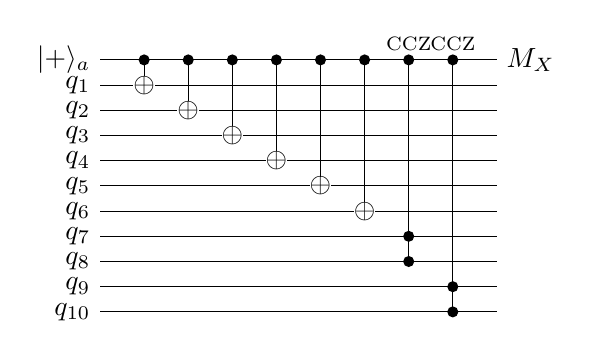
\begin{tikzpicture}[x=0.56cm,y=0.32cm]
\draw (0,0)--(9,0); \node[left] at (0,0) {$\ket{+}_a$};
\node[right] at (9,0) {$M_X$};
\foreach \i in {1,...,10} {
  \draw (0,-\i)--(9,-\i);
  \node[left] at (0,-\i) {$q_{\i}$};
}
\foreach \i in {1,...,6} {
  \draw (\i,0)--(\i,-\i);
  \fill (\i,0) circle (2pt);
  \node[fill=white,inner sep=0pt] at (\i,-\i) {$\oplus$};
}
\draw (7,0)--(7,-8); \foreach \y in {0,-7,-8} {\fill (7,\y) circle (2pt);}
\draw (8,0)--(8,-10); \foreach \y in {0,-9,-10} {\fill (8,\y) circle (2pt);}
\node[above] at (7,0) {\scriptsize CCZ};
\node[above] at (8,0) {\scriptsize CCZ};
\end{tikzpicture}

    \caption{Ancilla-based measurement circuit for a dressed stabilizer $S^{\rd}_{X;v}$: six controlled-$X$ gates for the Pauli part and two CCZ gates for the CZ dressing [Eq.~\eqref{eq:czlist}].}
    \label{fig:xstab_circuit}
\end{figure}

%=====================================================================
\section{Non-Commutativity of the Dressed Stabilizers}
\label{sec:noncomm}

\paragraph{Commutator.}
Let $S_A=X^{s_A}(-1)^{q_A}$ and $S_B=X^{s_B}(-1)^{q_B}$ be two dressed stabilizers. Applying Eq.~\eqref{eq:generic} twice,
\begin{align}
  S_AS_B\ket{a}&=(-1)^{q_B(a)+q_A(a+s_B)}\ket{a+s_A+s_B},\nonumber\\
  S_BS_A\ket{a}&=(-1)^{q_A(a)+q_B(a+s_A)}\ket{a+s_A+s_B},
\end{align}
so that $S_AS_B=S_BS_A\,(-1)^{\Delta_{AB}(a)}$ with
\begin{equation}
  \Delta_{AB}(a)=\big[q_A(a+s_B)+q_A(a)\big]+\big[q_B(a+s_A)+q_B(a)\big].
  \label{eq:delta}
\end{equation}
Because $q_A$ and $q_B$ are bilinear, $\Delta_{AB}$ is an affine function of $a$: if $q_A(a)=\sum_{(i,j)\in P_A}a_ia_j$, then $q_A(a+s_B)+q_A(a)=\sum_{(i,j)\in P_A}\big(s_{B,i}a_j+a_is_{B,j}+s_{B,i}s_{B,j}\big)$.

\paragraph{Worked example.}
Take $A=(\rd,(0,0))$ and $B=(\gr,(0,0))$ at $L=3$. The shift $s_B$ flips the green bits on the six edges of Eq.~\eqref{eq:star}, two of which, $\eh{0,0}$ and $\ev{0,0}$, appear in $q_A$ [Eq.~\eqref{eq:qexample}]. Hence $q_A(a+s_B)+q_A(a)=a_\bl(\ev{1,0})+a_\bl(\eh{0,1})$. In the same way $s_A$ flips the red bits on $\eh{2,0}$ and $\ev{0,2}$ that appear in $q_B$, so $q_B(a+s_A)+q_B(a)=a_\bl(\ev{0,0})+a_\bl(\eh{0,0})$. Adding,
\begin{align}
  \Delta_{AB}(a)&=a_\bl(\eh{0,0})+a_\bl(\ev{1,0})+a_\bl(\eh{0,1})+a_\bl(\ev{0,0})\nonumber\\
  &=(da_\bl)(\tlo{0,0})+(da_\bl)(\tup{0,0}),
  \label{eq:deltaexample}
\end{align}
the parity of the blue bits around the boundary of the unit square at the origin (the diagonal $\ed{0,0}$ appears in both triangles and cancels). Therefore
\begin{equation}
  S_AS_B=S_BS_A\,S^\bl_{Z;\tlo{0,0}}\,S^\bl_{Z;\tup{0,0}}.
\end{equation}

\paragraph{General rule.}
For the cup-product dressing, $\Delta_{AB}$ is always a sum of plaquette constraints: there is a set of faces $F_{AB}$ such that
\begin{equation}
  S_AS_B=S_BS_A\prod_{f\in F_{AB}}S^{c_f}_{Z;f}.
  \label{eq:commutator}
\end{equation}
Checks of the same color always commute, because $s_B$ then flips bits of a color that does not occur in $q_A$. Evaluating Eq.~\eqref{eq:delta} for all pairs as above, we find that on our lattice $F_{AB}$ is non-empty for exactly three pairs per unit square $(x,y)$, namely
\begin{align}
  S^\rd_{X;(x,y)}\ \&\ S^\gr_{X;(x,y)}&:\ \text{blue faces of square }(x,y),\nonumber\\
  S^\rd_{X;(x,y)}\ \&\ S^\bl_{X;(x+1,y+1)}&:\ \text{green faces of square }(x,y),\label{eq:pairs}\\
  S^\gr_{X;(x+1,y+1)}\ \&\ S^\bl_{X;(x+1,y+1)}&:\ \text{red faces of square }(x,y),\nonumber
\end{align}
where ``faces of square $(x,y)$'' means $F_{AB}=\{\tlo{x,y},\tup{x,y}\}$. All other pairs commute identically. We verified Eq.~\eqref{eq:commutator} numerically for all pairs at $L=3,4,5$: the number of non-commuting pairs is $3L^2$ (27 of the 351 pairs at $L=3$), and the constant term of $\Delta_{AB}$ always vanishes. Consequently the $X$-stabilizers commute on the flat subspace, as required for the code to be well defined~\cite{kobayashi2025clifford}, but \emph{two dressed checks anticommute on any state that carries an odd number of fluxes on $F_{AB}$}, i.e.\ a flux of the relevant color on exactly one of the two triangles of the square.

\paragraph{An $X$ error randomizes dressed measurements.}
Let $(q_1,q_2)$ be one of the CZ pairs of a check $S$. Because $X_{q_1}(-1)^{q(a)}X_{q_1}=(-1)^{q(a+\mathbf 1_{q_1})}=(-1)^{q(a)}Z_{q_2}$,
\begin{equation}
  X_{q_1}\,S\,X_{q_1}=S\,Z_{q_2}.
  \label{eq:dress}
\end{equation}
For example, the error $X^\gr_{\eh{0,0}}$ hits one qubit of a CZ pair of $S^\rd_{X;(0,0)}$ [Eq.~\eqref{eq:example}], and $X^\gr_{\eh{0,0}}S^\rd_{X;(0,0)}X^\gr_{\eh{0,0}}=S^\rd_{X;(0,0)}Z^\bl_{\ev{1,0}}$. In the measurement circuit the same relation reads $\mathrm{CCZ}_{a,q_1,q_2}X_{q_1}=X_{q_1}\mathrm{CZ}_{a,q_2}\mathrm{CCZ}_{a,q_1,q_2}$: the residual operator is an ancilla--data CZ, not a Pauli error. Now let $\ket{\psi}$ be a code state and consider the erroneous state $X_{q_1}\ket{\psi}$. Measuring $S$ with outcome $(-1)^m$ gives
\begin{align}
  \Pr(m)&=\tfrac12\big(1+(-1)^m\bra{\psi}Z_{q_2}\ket{\psi}\big)=\tfrac12,\\
  \frac{I+(-1)^mS}{2}X_{q_1}\ket{\psi}&=X_{q_1}\,\frac{I+(-1)^mZ_{q_2}}{2}\ket{\psi},
  \label{eq:collapse}
\end{align}
where we used $S\ket{\psi}=\ket{\psi}$, $[S,Z_{q_2}]=0$, and $\bra{\psi}Z_{q_2}\ket{\psi}=0$. The last equality holds because $Z_{q_2}$ anticommutes with the checks of its own color at the two ends of its edge; in the example, $Z^\bl_{\ev{1,0}}$ anticommutes with $S^\bl_{X;(1,0)}$ and $S^\bl_{X;(1,1)}$. The outcome is a fair coin and the post-measurement state is a superposition of ``no error'' and ``$Z_{q_2}$'', not a state with a definite $Z$ error.

\paragraph{Repeated measurements while a flux is present.}
Suppose $S_A$ and $S_B$ anticommute on the current state, i.e.\ a flux sits on $F_{AB}$. In the example above, $X^\gr_{\eh{0,0}}$ creates green fluxes on $\tlo{0,0}$ and $\tup{0,2}$, so by Eq.~\eqref{eq:pairs} the pairs $\big(S^\rd_{X;(0,0)},S^\bl_{X;(1,1)}\big)$ and $\big(S^\rd_{X;(0,2)},S^\bl_{X;(1,0)}\big)$ now anticommute. After $S_A$ is measured with outcome $m_A$, the state is an eigenstate of $S_A$ and $\langle S_B\rangle=\langle S_AS_BS_A\rangle=-\langle S_B\rangle=0$; after $S_B$ is measured, $\langle S_A\rangle=0$ by the same argument. In the sequence $A\to B\to A$, therefore,
\begin{equation}
  \Pr\big(m_A^{(2)}=m_A^{(1)}\big)=\tfrac12,
  \label{eq:aba}
\end{equation}
and this re-randomization repeats in every round for as long as the flux survives. The $X$-stabilizer syndrome near a flux is thus a sequence of fair coins whose statistics depend on the measurement order and on the flux lifetime. A decoder sees these coins as a burst of measurement errors and, when the flux is finally removed, as $Z$-type (charge) errors whose presence was decided by the last measurements [Eq.~\eqref{eq:collapse}].

\paragraph{Why the previous surrogate could not represent this.}
The previous study~\cite{haga2026aqis} measured the bare checks $\bar S_A=X^{s_A}$ on the product state $\ket{+}^{\otimes n}$ and applied, in every round and independently of everything else, $Z$ errors with probability $r=\kappa cp$ to each qubit of every dressed pair (Sec.~\ref{sec:noise} gives the exact definitions). This model differs from Eqs.~\eqref{eq:collapse}--\eqref{eq:aba} in four respects.
\begin{enumerate}[leftmargin=*,itemsep=0pt]
\item \emph{Commutation.} The bare checks commute with each other, so no measurement ever changes the statistics of another. Eq.~\eqref{eq:aba} is replaced by $\Pr(m_A^{(2)}\neq m_A^{(1)})=O(r)$, regardless of whether a flux is present.
\item \emph{Correlations in space and time.} In the real code the randomization occurs only near fluxes and lasts for their lifetime; in the surrogate it is spread uniformly over all pairs and all rounds with a fixed rate. No fixed independent injection rate reproduces the history-dependent measurement statistics. Persistent flux can cause repeated randomization, while residual diagonal Clifford errors can also cause random outcomes after the flux is removed.
\item \emph{No flux dynamics.} Because bare checks commute with $X$ errors, the surrogate had no reason to measure or correct fluxes, and none were corrected. In the real code uncorrected fluxes accumulate, their number grows with the number of rounds $R\propto L$, and flux configurations with odd parity on a relevant commutator support cause repeated randomization of the corresponding checks. Residual diagonal Clifford errors can survive flux removal. A faithful $X$-stabilizer memory for this code must therefore include flux correction during the run.
\item \emph{Calibration.} $\kappa$ was fitted to the firing rate of a single check measured twice ($A\to A$) starting from $\ket{+}^{\otimes n}$. This marginal statistic is blind to the correlations between different checks in Eq.~\eqref{eq:aba}, so agreement of the calibration curves did not imply agreement of the joint syndrome statistics that the decoder uses.
\end{enumerate}
In addition, the circuit-level model of Ref.~\cite{haga2026aqis} aggregated all gate noise into per-round data noise and a readout flip probability $p$, whereas in the actual circuit of Fig.~\ref{fig:xstab_circuit} the ancilla collects faults from six controlled-$X$ gates and two CCZ gates (Sec.~\ref{sec:noise}), and ancilla faults spread into partial stabilizers (``hook'' errors). Finally, the green dressing pairs in the previous implementation had the two colors interchanged relative to Eq.~\eqref{eq:czlist}: $S^\gr_{X;(x,y)}$ contained $\mathrm{CZ}(\bl\,\eh{x-1,y},\rd\,\ev{x,y})\,\mathrm{CZ}(\bl\,\ev{x,y-1},\rd\,\eh{x,y})$, i.e.\ blue on $e_{01}$ and red on $e_{12}$. With that assignment 90 of the 351 check pairs at $L=3$ fail to commute even on flat configurations, so the checks did not define the $\mathbb{D}_4$ code. We use Eq.~\eqref{eq:czlist} throughout.

%=====================================================================
\section{Exact Simulation of Dressed Measurements}
\label{sec:method}

\paragraph{Flat configurations in coordinates.}
On the torus, every flat configuration of one color with vertical holonomy fixed to zero can be written as $a_c=d\mu_c+h_c\,\eta$. Here $\mu_c$ assigns a bit to every vertex, $(d\mu_c)(e)=\mu_c(v)+\mu_c(w)$ for an edge $e=(v\to w)$, $h_c\in\GF$, and $\eta$ is the indicator of the edges $\eh{0,y}$ and $\ed{0,y}$ ($y=0,\dots,L-1$), i.e.\ of the edges that cross the vertical line between the columns $x=0$ and $x=1$. Fixing $\mu_c(0,0)=0$ makes the parametrization one-to-one. The bit $h_c$ is the holonomy along the horizontal loop $\gamma_x=\{\eh{0,0},\eh{1,0},\dots,\eh{L-1,0}\}$: the logical operator $Z^c(\gamma_x)=\prod_{x'}Z^c_{\eh{x',0}}$ has eigenvalue $(-1)^{h_c}$, because $d\mu_c$ sums to zero around any closed loop and $\eta$ meets $\gamma_x$ once. We fix the holonomy along the vertical direction to zero. The space $C_0$ of configurations that store the logical information is therefore parametrized by $t=(\mu_\rd,\mu_\gr,\mu_\bl,h_\rd,h_\gr,h_\bl)\in\GF^k$ with $k=3(L^2-1)+3=3L^2$ (27 at $L=3$), and $a=Mt$ for a fixed $n\times k$ binary matrix $M$. The shift $s_A=d\tilde v$ of every check lies in $C_0$, since it corresponds to $\mu_c=\tilde v$ (or, for $v=(0,0)$, to $\mu_c=\sum_{w\neq(0,0)}\tilde w$, which has the same coboundary).

\paragraph{Twisted-frame representation.}
Let $\ket{\psi_0}=\sum_{b\in C_0}(-1)^{\phi_0(b)}\ket{b}$ be a code state. Because $S\ket{\psi_0}=\ket{\psi_0}$ for every dressed check,
\begin{equation}
  \phi_0(b+s)+\phi_0(b)=q(b+s)\qquad(b\in C_0).
  \label{eq:stabcond}
\end{equation}
The phase $\phi_0$ itself is cubic in $b$, and we never need to compute it.

\begin{proposition}
Let $\ket{\psi}$ be obtained from $\ket{\psi_0}$ by any sequence of Pauli operators, CZ gates, measurements of $Z$-plaquettes, and projective measurements of dressed $X$-stabilizers (possibly multiplied by a Pauli-$Z$ operator on a dressing qubit). Then, up to normalization,
\begin{equation}
  \psi(a)=(-1)^{\phi_0(a+x)+Q(a+x)}\,\mathbf{1}\big[a+x\in B\big],
  \label{eq:tf}
\end{equation}
where $x\in\GF^{n}$ is the accumulated Pauli-$X$ frame, $B\subseteq C_0$ is an affine subspace, and $Q$ is a quadratic form over $\GF$. The phase of the state is therefore the cubic phase $\phi_0$ of the initial code state plus the quadratic form $Q$; only $Q$ changes during the protocol. Every measurement outcome has probability $0$, $\tfrac12$ or $1$.
\end{proposition}

Here an \emph{affine subspace} is the solution set $\{b=Mt:\ Gt=\rho\}$ of a system of linear equations over $\GF$, and a \emph{quadratic form} is a function $Q(b)=\sum_{i<j}W_{ij}t_it_j+\sum_i\ell_it_i\bmod2$ of the coordinates $t$. The frame $x$ records which $X$ errors (and corrections) have been applied, so that $b=a+x$ is the configuration ``seen through'' the frame.

\begin{proof}
Pauli $X$ errors only change $x$. $Z$ errors and CZ gates multiply $\psi$ by $(-1)^{\ell(a)}$ or $(-1)^{a_ia_j}$ [Eq.~\eqref{eq:cz}] and add a linear or quadratic term to $Q$. A plaquette measurement returns $(dx)(f)$ deterministically because $B\subseteq C_0$ is flat. For a dressed check, write $b=a+x$. For points with both $b\in B$ and $b+s\in B$ (so the amplitude ratio is defined), Eq.~\eqref{eq:stabcond} gives
\begin{equation}
  \frac{(S\psi)(a)}{\psi(a)}=(-1)^{f(b)},\quad f(b)=q(b+s+x)+q(b+s)+Q(b+s)+Q(b),
  \label{eq:f}
\end{equation}
The polynomial $f$ extends to $C_0$ and is affine in $b$ because $q$ and $Q$ are at most quadratic. When $b+s\notin B$, the shifted amplitude is zero and we use the disjoint-support argument in case (ii), not the amplitude ratio. (i) If $s$ lies in the direction space of $B$, the outcome is deterministic when $f$ is constant on $B$; otherwise it is uniform and $B$ is restricted to $\{f(b)=m\}$. (ii) If $s$ does not lie in the direction space of $B$, then $B$ and $B+s$ are disjoint, $\langle S\rangle=0$, the outcome is uniform, $B\to B\cup(B+s)$, and $Q\to Q+\lambda(b)\,(f(b)+m)$, where $\lambda$ is the affine indicator of $B+s$. Both updates preserve Eq.~\eqref{eq:tf}. An extra $Z$ factor adds a linear term to $f$.
\end{proof}

\paragraph{Example.}
Start from $\ket{\psi_0}$ ($x=0$, $B=C_0$, $Q=0$) at $L=3$ and apply $X^\gr_{\eh{0,0}}$, so that $x=\mathbf 1_{(\eh{0,0},\gr)}$. Measuring $A=(\rd,(0,0))$: $s_A\in C_0$, and since $q_A$ does not depend on red bits, Eqs.~\eqref{eq:qexample} and \eqref{eq:f} give $f(b)=q_A(b+x)+q_A(b)=b_\bl(\ev{1,0})$. This is not constant on $B$, so case (i) applies: the outcome $m$ is uniform and $B$ is restricted to $b_\bl(\ev{1,0})=m$, which is Eq.~\eqref{eq:collapse} in this representation. If $S^\bl_{X;(1,1)}$ is measured next, its shift flips $b_\bl(\ev{1,0})$ (the edge $\ev{1,0}$ ends at $(1,1)$), so it does not lie in the direction space of the restricted $B$; case (ii) applies and this outcome is again a fair coin. This is the anticommuting pair of Eq.~\eqref{eq:pairs} for the green flux on $\tlo{0,0}$.

Case (ii) of the proof is thus the non-commutativity of Sec.~\ref{sec:noncomm}: it occurs precisely when an earlier measurement has restricted $B$ in a direction that the present check moves. We store $x$, a row-reduced basis of the constraints that define $B$, and $Q$ as bit-packed matrices of size $k\times k$ with $k=3L^2$. A measurement then costs $O(k^2)$ bit operations, and a full shot at $L=7$, including decoding, takes a few milliseconds on one CPU core. The representation is an exact, state-level version of the ``twisted-error'' sampling discussed in Refs.~\cite{davydova2025knots,magdalena2026}. It is also a special case of the Clifford-stabilizer simulation of Takada, Bartlett and Williamson~\cite{takada2026exact}: the group commutator of two dressed checks is the product of $Z$-plaquettes of Eq.~\eqref{eq:commutator}, so every dressed measurement is effectively commuting or anticommuting with the current stabilizers, and their Pauli-proxy method applies. Section~\ref{sec:validation} compares the two implementations.

\paragraph{Circuit-level faults.}
For circuit-level noise we use the circuit of Fig.~\ref{fig:xstab_circuit} with a native CCZ gate. A Pauli fault anywhere in the circuit is propagated to the end of the circuit through the remaining controlled-$X$ and CCZ gates. By Eq.~\eqref{eq:dress}, and because $\mathrm{CCZ}$ maps $X$ on one of its qubits to $X$ times a CZ on the other two, the propagated fault is a Pauli operator times CZ gates. The faulty measurement therefore acts as a projection onto an eigenspace of $S$, followed by CZ and Pauli errors on the data and possibly a flipped outcome, all of which preserve Eq.~\eqref{eq:tf}. (An ancilla--data CZ, which would turn the measured operator into $S$ times a $Z$ on a dressing qubit, would require an $X$ on a dressing qubit before its CCZ; no fault inside the circuit produces one, as the fault tables confirm. The ancilla--data CZ of Eq.~\eqref{eq:dress} caused by an $X$ error \emph{already present} on the data is accounted for exactly by the frame $x$ in Eq.~\eqref{eq:f}.) Multiple faults in one circuit are composed in time order. Faults inside a $T$-gate decomposition of the CCZ produce non-Clifford error operators and are outside the present method.

%=====================================================================
\section{Memory Protocol with Just-in-Time Flux Correction}
\label{sec:protocol}

\paragraph{Initial state and rounds.}
We start from the noiseless code state that is an equal superposition over the $2^3$ values of $(h_\rd,h_\gr,h_\bl)$ (Sec.~\ref{sec:method}); it is sensitive to the three logical string operators $Z^c(\gamma_x)$ that wind horizontally around the torus. Each of the $R$ rounds consists of (1) data noise, (2) measurement of all $6L^2$ $Z$-plaquettes, (3) JIT flux decoding and immediate physical $X$ correction, and (4) measurement of the $3L^2$ dressed $X$-checks color by color ($\rd\to\gr\to\bl$).

\paragraph{Just-in-time flux decoding.}
A matching decoder that waits for the full syndrome history is not appropriate here: a surviving flux can make the corresponding dressed measurements random [Eq.~\eqref{eq:aba}]. Fluxes must be removed during the run using only the plaquette outcomes observed so far. This is the just-in-time idea of Bombin~\cite{bombin2018jit} and Brown~\cite{brown2020jit}, which is also the decoding strategy proposed for this code~\cite{kobayashi2025clifford} and for related non-Abelian codes~\cite{davydova2025knots,magdalena2026}. Our implementation is a minimum-weight-matching variant, run separately for each color.
\begin{enumerate}[leftmargin=*,itemsep=0pt]
\item At round $t$ the measured plaquette syndrome $\sigma_t$ is corrected for the fluxes created by all previously applied corrections $C_{<t}$, $\sigma'_t=\sigma_t\oplus\partial C_{<t}$. Detection events are the plaquettes with $\sigma'_t\neq\sigma'_{t-1}$. They are added to the set $U$ of unresolved events, each labelled by its time.
\item We run minimum-weight perfect matching (PyMatching~\cite{higgott2025pymatching}) on $U$ over the space--time graph of layers $0,\dots,t$. Space-like edges connect two triangles that share an edge (e.g.\ $\tlo{x,y}$ and $\tup{x,y}$, which share $\ed{x,y}$) with weight $w_s=\ln[(1-p_X)/p_X]$, and time-like edges connect consecutive layers with weight $w_t=\ln[(1-p_M)/p_M]$. Here $p_X$ and $p_M$ are the probabilities of an $X$-type data error and of a flipped plaquette outcome per round. Every node of layer $t$ is joined to a ``future'' boundary with weight $w_t$, so that leaving an event born at time $\tau$ unresolved costs $w_t(t-\tau+1)$. When the plaquette outcomes are perfect ($p_M=0$, code-capacity noise) the future boundary is omitted, so that every event is matched in space at once (on the torus the number of fluxes of each color is even, so a perfect matching always exists). For the sizes studied here this changes no decision of the decoder.
\item For every pair of \emph{events} matched to each other we immediately apply $X^c$ on the edges crossed by a shortest path between their triangles in the dual lattice (whose nodes are triangles and whose links are shared edges), and remove both from $U$. Events matched to the future boundary stay in $U$ and are reconsidered in the next round.
\item The corrections are applied before the dressed checks of the same round.
\end{enumerate}
The waiting cost in step 2 encodes the trade-off at the heart of JIT decoding. A single $X$ error creates two adjacent fresh events whose pairing cost $w_s$ is smaller than the waiting cost $2w_t$, so it is corrected at once, before any dressed check can see the flux. An isolated event, typically a flipped plaquette outcome, has no partner and waits for the next round, where its partner appears at the same place and is matched along a time-like edge without any correction. If instead the boundary is placed at the current layer at zero cost, every flux survives at least one layer of dressed measurements. In pilot runs of the phenomenological model at $p=2\%$ this choice gave logical failure rates of \blue{0.29, 0.42 and 0.58 [pilot runs]} for $L=3,5,7$, i.e.\ no error suppression in the sizes we tested. Controlling the flux lifetime is therefore essential for the $X$-stabilizer threshold of this code, and a model that does not correct fluxes cannot estimate it.

\paragraph{Termination.}
After the last noisy round we measure all plaquettes perfectly and close the remaining fluxes by minimum-weight matching. If the residual $X$ frame is homologically non-trivial, the shot is counted as a failure of the flux sector (a logical error detected by the $Z$-stabilizers). Otherwise the frame is a coboundary, $x_c=d\mu_c$, and we remove it by applying the stabilizers $S^c_{X;v}$ for all $v$ with $\mu_c(v)=1$ as unitaries; this leaves the logical state unchanged. A final round of perfect dressed measurements follows.

\paragraph{Charge decoding and logical failure.}
Detection events for the charges are changes of the dressed-check outcomes between consecutive rounds. Charges of different colors are decoded independently by PyMatching on a space--time graph whose weights are taken from the detector error model of a bare-check Stim circuit with the appropriate per-round $Z$-type data error rate and outcome-flip rate (Sec.~\ref{sec:noise}). The prior can additionally contain the $r=\kappa_{\mathrm{dec}}cp$ pair channel of Ref.~\cite{haga2026aqis}. Here $\kappa_{\mathrm{dec}}$ only affects the decoder, not the simulated physics. We use $\kappa_{\mathrm{dec}}=0.5$ for code capacity, $0$ for phenomenological noise, and $0.1$ for circuit-level noise ($0$ for the earlier version of the circuit-level model). These values minimize the charge failure rate at the largest size of a scan near the crossing ($L=3,5,7$, $2\times10^4$ shots per point, seeds different from the production runs; for circuit-level noise also $L=7,9$ at two further values of $p$). Within the scanned values the differences are within the statistical errors for code capacity ($\kappa_{\mathrm{dec}}\ge0.25$) and phenomenological noise ($\kappa_{\mathrm{dec}}\le0.1$), whereas for circuit-level noise $\kappa_{\mathrm{dec}}=0.1$ lowers the failure rate at $L=9$, $p=0.15\%$ from $3.3\%$ to $2.8\%$. The decoder was not optimized further. We then apply a canonical correction compatible with the final syndrome (strings of $Z^c$ along a fixed spanning tree rooted at $(0,0)$), combine it with the homology class predicted by the decoder from the parity of the correction on the edges $\eta$, and compute from the sector phases of the final state its fidelity $F$ with the initial logical state; the shot fails with probability $1-F$.

\paragraph{Failure metrics.}
We report three failure probabilities: the flux-sector failure rate $P_{\mathrm{flux}}$, the combined rate $P_{\mathrm{comb}}$ of a failure in either sector, and the \emph{charge-sector} (i.e.\ $X$-stabilizer) failure rate
\begin{equation}
  P_{\mathrm{charge}}=\Pr(\text{charge failure}\mid\text{flux success}),
\end{equation}
which is the quantity whose crossing we call the $X$-stabilizer threshold. Two restrictions should be kept in mind. First, $P_{\mathrm{charge}}$ is conditioned on the success of the flux sector, and whether the flux sector failed is decided with the true error frame of the simulation; it is an analysis quantity, not a post-selection available in an experiment. We therefore always report $P_{\mathrm{flux}}$ and $P_{\mathrm{comb}}=P_{\mathrm{flux}}+(1-P_{\mathrm{flux}})P_{\mathrm{charge}}$ as well. Second, the initial state is a superposition of the eight holonomy sectors along one direction, so $P_{\mathrm{charge}}$ is a failure rate for this family of logical states and this protocol, not a bound on an arbitrary logical channel of the 22-dimensional code space. All rates carry $95\%$ Agresti--Coull intervals~\cite{agresti1998}.

%=====================================================================
\section{Noise Models: Previous and Present Definitions}
\label{sec:noise}

All models are parametrized by a single physical error rate $p$. $\mathtt{DEPOLARIZE1}(p)$ applies $X$, $Y$ or $Z$ with probability $p/3$ each, and $\mathtt{DEPOLARIZE2}(p)$ applies each of the 15 non-identity two-qubit Paulis with probability $p/15$. An ``$X$-type'' error is $X$ or $Y$ (it creates fluxes), and a ``$Z$-type'' error is $Z$ or $Y$ (it creates charges, i.e.\ flips dressed checks). The noise models have the same names as in Ref.~\cite{haga2026aqis}, but their definitions have changed, in two ways: what is simulated (the dressed measurement itself instead of a surrogate), and, for the code-capacity model, which noise is included. Table~\ref{tab:noise} summarizes both versions.

\paragraph{Previous definitions~\cite{haga2026aqis}.}
All three models were Stim circuits on $\ket{+}^{\otimes n}$ in which, in each of $R=L$ rounds, the bare checks $X^{s_A}$ were measured by noisy multi-qubit Pauli measurements (\texttt{MPP}); the $Z$-plaquettes were not measured. Before each round of \texttt{MPP}, every CZ pair $(q_1,q_2)$ received the ``kickback'' channel $\mathtt{PAULI\_CHANNEL\_2}$ with probabilities $r(1-r)$, $r(1-r)$, $r^2$ for $IZ$, $ZI$, $ZZ$, i.e.\ an independent $Z$ on each qubit with probability $r$. The models differed only in the data noise and in $r$:
\begin{itemize}[leftmargin=*,itemsep=0pt]
\item \emph{Depolarizing}: $\mathtt{DEPOLARIZE1}(p)$ on all data qubits and outcome flips with probability $p$ in every round, and a noisy final data readout. $r=\kappa cp$ with $c=2/3$, $\kappa=0.5$, divided between the two CZ pairs that share each dressing qubit, so $r=p/6$ per pair and about $p/3$ per dressing qubit and round.
\item \emph{Phenomenological}: identical, except $r=\kappa p$ with $\kappa=0.25$ per pair ($c=1$), i.e.\ about $p/2$ per dressing qubit and round. Up to the value of $r$ these two models are the same physical model.
\item \emph{Circuit-level} (aggregated): the gate error rates below were summed into per-round data noise $\mathtt{DEPOLARIZE1}(p_{\mathrm{rd}})$ with $p_{\mathrm{rd}}=1-(1-0.4p)(1-0.35p)(1-\tfrac83p)\approx3.4p$ (idle, one-qubit gates, and four controlled-$X$ gates), outcome flips with probability $p$, and $r=\kappa(p_{2q}+3p_{\mathrm{nc}})=0.6\times4p$ per pair ($c=4$, counting one two-qubit and three non-Clifford locations per CCZ).
\end{itemize}
The logical failure rate was the probability that any of six logical observables (three colors, two directions) was flipped.

\paragraph{Present definitions.}
All models simulate the dressed checks exactly (Sec.~\ref{sec:method}) within the protocol of Sec.~\ref{sec:protocol}: noiseless initial code state, $Z$-plaquettes measured and fluxes corrected in every round, ideal termination, and failure metric $P_{\mathrm{charge}}$. There is no $\kappa$ in the simulated physics; the randomization of Sec.~\ref{sec:noncomm} arises by itself.
\begin{itemize}[leftmargin=*,itemsep=0pt]
\item \emph{Code-capacity depolarizing}: one round ($R=1$) in which $\mathtt{DEPOLARIZE1}(p)$ acts once on all $9L^2$ data qubits, followed by perfect plaquette and dressed measurements. Unlike before, there are no measurement errors. The previous definition (outcome flips with probability $p$, $R=L$) coincides with our phenomenological model.
\item \emph{Phenomenological}: $R=L$ rounds. In each round $\mathtt{DEPOLARIZE1}(p)$ acts on all data qubits, and every plaquette outcome and every dressed-check outcome is recorded with a flip of probability $p$ (the state is projected according to the true outcome).
\item \emph{Circuit-level}: $R=L$ rounds of the gate-resolved circuits with the standard circuit-level Pauli noise of Ref.~\cite{takada2026exact} (App.~A2): after every $k$-qubit gate a $k$-qubit depolarizing channel of probability $p$, i.e.\ $\mathtt{DEPOLARIZE2}(p)$ after each controlled-$X$ gate and, after each \emph{native} CCZ gate, the three-qubit depolarizing channel that applies each of the 63 non-identity three-qubit Paulis with probability $p/63$; a preparation is followed, and a measurement preceded, by a flip with probability $p$; there is no idle noise, and the JIT corrections are noiseless Pauli-frame updates. Each plaquette $S^c_{Z;\Delta}$ is measured with a fresh ancilla prepared in $\ket0$ and three controlled-$X$ gates (data$\to$ancilla); each dressed check uses the circuit of Fig.~\ref{fig:xstab_circuit} with the ancilla prepared and measured in the $X$ basis (the Hadamard gates are part of preparation and measurement). Every fault is propagated through the rest of its circuit exactly (Sec.~\ref{sec:method}), which produces hook errors automatically. This is the same noise model as in our code-switching study of the same code, so that $p$ has the same meaning in both.
\end{itemize}
To first order in $p$, the actual circuit flips each dressed-check outcome with probability about $6.2p$ and gives each data qubit a $Z$-type error with probability about $5.6p$ per round (counting a data--data CZ error as a $Z$ on either qubit with probability $\tfrac12$).
An earlier version of the present circuit-level model (used for the $10^4$-shot runs quoted as ``v7 definition'' below) inherited the gate error weights of Ref.~\cite{haga2026aqis}: reset $\mathtt{DEPOLARIZE1}(0.6p)$, Hadamard and JIT corrections $\mathtt{DEPOLARIZE1}(0.35p)$, idle $\mathtt{DEPOLARIZE1}(0.4p)$ once per round, and $\mathtt{DEPOLARIZE1}(p)$ on each of the three qubits of a CCZ instead of the three-qubit channel (a first-order fault rate of $3p$ per CCZ). Its first-order rates are $6.4p$ and $6.3p$, and its crossings lie at nearly the same place as those of the present model (Table~\ref{tab:thresholds}). These rates, obtained from the fault tables of the circuit, set the weights of the circuit-level charge decoder. For the other two models the decoder uses the data error rate $\tfrac23p$ and a flip probability $\max(p_M,0.5p)$, the floor keeping time-like edges in the graph when $p_M=0$.

\begin{table*}[t]
\centering
\caption{Noise models of the previous study~\cite{haga2026aqis} and of this work. $p_{2q}$, $p_{\mathrm{nc}}$: error rates of two-qubit and non-Clifford gates; both are $p$ in all models. The previous circuit-level model and the earlier (``v7'') version of the present one used the gate error weights reset $0.6p$, one-qubit gate $0.35p$, two-qubit gate $p$, CCZ $p$ on each qubit, idle $0.4p$, readout $p$; the present one uses the uniform model of Ref.~\cite{takada2026exact}.}
\label{tab:noise}
\small
\renewcommand{\arraystretch}{1.15}
\begin{tabular}{p{0.15\linewidth}p{0.39\linewidth}p{0.39\linewidth}}
\toprule
 & previous~\cite{haga2026aqis} & present \\
\midrule
what is measured & bare checks $X^{s_A}$ (Clifford surrogate, Stim), $R=L$ rounds; no $Z$-plaquettes; initial state $\ket{+}^{\otimes n}$ & dressed checks $X^{s_A}(-1)^{q_A}$ exactly, and $Z$-plaquettes; JIT flux correction; noiseless code state, ideal termination \\
effect of the dressing & independent $Z$ on each dressing qubit with probability $r=\kappa cp$ per pair and round & arises from the exact measurement (no fitted parameter) \\
\midrule
depolarizing / code capacity & $\mathtt{DEPOLARIZE1}(p)$ and outcome flips $p$ per round, $R=L$; $c=\tfrac23$, $\kappa=0.5$ & $\mathtt{DEPOLARIZE1}(p)$ once; perfect measurements ($R=1$) \\
phenomenological & as above; $c=1$, $\kappa=0.25$ & $\mathtt{DEPOLARIZE1}(p)$ per round; plaquette and dressed-check outcome flips $p$; $R=L$ \\
circuit-level & aggregated: data $\mathtt{DEPOLARIZE1}(\approx3.4p)$ per round, outcome flips $p$; $c=4$, $\kappa=0.6$ & gate-resolved circuits (Fig.~\ref{fig:xstab_circuit}) with native CCZ; $k$-qubit depolarizing $p$ after every $k$-qubit gate, preparation and measurement flips $p$, no idle noise~\cite{takada2026exact}; faults propagated exactly; effective outcome flip $\approx6.2p$ \\
\midrule
failure metric & any of 6 logical observables flipped & $P_{\mathrm{charge}}$ (Sec.~\ref{sec:protocol}) \\
\bottomrule
\end{tabular}
\end{table*}

\paragraph{Control experiments.}
To compare the full dressed model with two specified control models, we repeat the simulations with identical noise, protocol, and decoders in two variants. \emph{Untwisted}: the CZ dressing is removed ($q_A\equiv0$), which turns the code into three independent $\mathbb{Z}_2$ toric codes; in the circuit-level model the CCZ gates are then absent as well. \emph{$\kappa$-injection}: untwisted, plus the independent pair-$Z$ noise $r=\kappa cp$ of Ref.~\cite{haga2026aqis} (with the previous values of $c$ and $\kappa$) applied before every layer of checks. This embeds the previous approximation in the present protocol. For the $\kappa$-injection variant we keep the previous definition of $r$ (with the previous gate error weights) in all versions of the circuit-level model.

%=====================================================================
\section{Validation at \texorpdfstring{$L=3$}{L=3}}
\label{sec:validation}

The Proposition is an exact algebraic statement. To guard against implementation errors we compare the sampler with an independent brute-force simulation of the same protocol at $L=3$. The brute-force simulation stores the state as a dense vector over the flat gauge configurations of the chosen sectors: $2^{25}$ amplitudes for one logical color and $2^{27}$ for three [$k=3L^2=27$, Sec.~\ref{sec:method}], computed with JAX~\cite{jax2018github} on a GPU. It applies every operation literally, including the two ancilla branches and every controlled-$X$ and CCZ gate of the circuit-level model. Driving both simulators with the same noise realization, all outcome probabilities along the tested trajectories agree to the single-precision rounding of the dense simulation (maximum deviation $1.1\times10^{-8}$, $1.9\times10^{-9}$ and $6.0\times10^{-8}$ for code-capacity, phenomenological and circuit-level noise), and so do the final logical fidelities (maximum deviation $1.2\times10^{-7}$). We checked 30 trajectories per noise model for one logical color and 10 for three; they contain 29, 162 and 295 (one color) and 10, 54 and 78 (three colors) outcomes of probability $\tfrac12$, so the agreement is not restricted to trivial trajectories. We further compare the logical failure rates of the two simulators obtained from independent samples (2000 dense and 50000 sampler shots at six values of $p$; Fig.~\ref{fig:validation}). They agree within statistical error: $\sum z^2=1.46$, $6.49$ and $7.24$ for 6 degrees of freedom (upper-tail probabilities $0.96$, $0.37$ and $0.30$) for the charge sector. These comparisons were made with the earlier (v7) circuit-level noise model; for the present one the trajectory comparison has so far been repeated on \blue{2} trajectories (31 random outcomes, maximum deviation $1.2\times10^{-7}$) \blue{[replace by the full GPU run, including the independent-sample comparison for three logical colors]}.

\paragraph{Comparison with the Clifford-stabilizer simulation at $L\le9$.}
The brute-force comparison is limited to $L=3$, while parts of the implementation depend on $L$ (bit packing, lattice geometry, decoding graphs). Agreement at $L=3$ is therefore numerical evidence that supports, but does not prove, the correctness of the runs at $L\ge5$. To test larger sizes we implemented the Pauli-proxy simulation of Ref.~\cite{takada2026exact} for the same memory experiment: the physical state is written as $E\,C\ket{\mathrm{frame}}$ with $C=\mathrm{diag}((-1)^{\phi_0})$, an error frame $E$ (Pauli $X$ frame times a diagonal Clifford operator) and a Pauli stabilizer state $\ket{\mathrm{frame}}$ propagated by Stim; a dressed check is measured as the Pauli operator obtained by conjugating it with $E$ and replacing its CZ factor by the identity, which is exact because of Eq.~\eqref{eq:stabcond}. This representation shares no code with the affine-subspace representation. Driven by the same noise realizations and the same decoders, the two simulators gave identical outcome probabilities and identical final fidelities (for all $2^3$ decoder corrections) on every trajectory we tested: 14\,400 trajectories at $L=3,5,7,9$ (2000, 1000, 400 and 200 per size) for code-capacity, phenomenological and circuit-level noise (both versions of the circuit-level model), containing $5.3\times10^6$ dressed measurements of which $4.2\times10^5$ had probability $\tfrac12$ (e.g.\ $3.2\times10^4$ for phenomenological noise at $L=9$). Deliberately removing the Pauli dressing, or the CZ part of the error frame, from the Pauli-proxy simulation makes the comparison fail within the first trajectories. The fault tables of the circuit-level model are shared by both simulators; their gate-level content is checked by the brute-force simulation at $L=3$.

\begin{figure*}[t]
  \centering
  \fbox{\rule{0pt}{50mm}\rule{0.82\linewidth}{0pt}}
  \caption{\blue{[Insert \texttt{d4\_v11\_validation\_L3\_<model>\_C\_<r|rgb>.pdf} from \texttt{D4\_v11\_validation.ipynb}, one panel per noise model.]} Validation at $L=3$: charge-sector failure probability versus $p$ from the brute-force state-vector simulation (squares) and from the twisted-frame sampler (circles). Error bars are $95\%$ confidence intervals.}
  \label{fig:validation}
\end{figure*}

%=====================================================================
\section{Results}
\label{sec:results}

\begin{figure*}[t]
  \centering
  \fbox{\rule{0pt}{50mm}\rule{0.82\linewidth}{0pt}}
  \caption{\blue{[Insert \texttt{d4\_v11\_X\_memory\_<model>\_twisted\_frame[\_uniform].pdf} from \texttt{D4\_v11\_main.ipynb}, one panel per noise model.]} Charge-sector ($X$-stabilizer) failure probability $P_{\mathrm{charge}}$ versus physical error rate $p$ for $L=3,5,7,9$. Error bars are $95\%$ Agresti--Coull intervals.}
  \label{fig:threshold}
\end{figure*}

Figure~\ref{fig:threshold} shows $P_{\mathrm{charge}}$ for the three noise models, and Table~\ref{tab:thresholds} lists the crossings of neighboring sizes with the 2.5--97.5\% range of the crossing over resampled data (failure counts redrawn from Jeffreys posteriors; only draws with a single crossing are used). This range describes the sampling variation of the crossing position, not a confidence interval for an asymptotic threshold. For phenomenological noise the crossings move to lower $p$ as $L$ grows, by $0.16$ and then $0.09$ percentage points. For circuit-level noise the $L=5$--$7$ and $7$--$9$ crossings also decrease, while the $L=3$ and $5$ curves nearly coincide around the crossing and give several crossings at the present statistics. For code-capacity noise the crossings lie between $9\%$ and $10.2\%$ and rise with $L$ in these data, but the curves cross at a shallow angle and the ranges overlap, so the $L$ dependence is not resolved. Crossings involving $L=3$ are also the most sensitive to the decoder prior. We therefore quote the crossing of the largest pair as a finite-size estimate,
\begin{equation}
  p_\times^{\,\mathrm{cc}}(7,9)\approx10.2\%,\quad
  p_\times^{\,\mathrm{pheno}}(7,9)\approx2.0\%,\quad
  p_\times^{\,\mathrm{circ}}(7,9)\approx\blue{0.19\%},
\end{equation}
and note that the phenomenological and circuit-level values are still drifting downward, so the asymptotic thresholds are expected to be somewhat lower. \blue{[Replace by the $10^5$-shot runs focused on the crossings; circuit-level with the present noise model.]}

\begin{table}[t]
\centering
\caption{Crossings of the $P_{\mathrm{charge}}$ curves of neighboring sizes, in units of $10^{-2}$ ($10^{-3}$ for circuit-level), from runs with $10^4$ shots per point and $L\le9$; in parentheses the 2.5--97.5\% range of the crossing over resampled data. The circuit-level rows give the earlier (v7) noise model and pilot runs of the present one ($L\le7$, $4\times10^3$ shots per point, $\kappa_{\mathrm{dec}}=0.1$); in the latter the $L=3$ curve is lowered most by the decoder prior, which moves the $L=3$--$5$ crossing down. \blue{[Replace by the $10^5$-shot runs.]}}
\label{tab:thresholds}
\small
\begin{tabular}{lccc}
\hline
model & $L=3$--$5$ & $5$--$7$ & $7$--$9$\\
\hline
code capacity & 9.24 (8.79--9.63) & 9.54 (8.85--10.24) & 10.15 (9.53--10.61)\\
phenomenological & 2.247 (2.174--2.302) & 2.088 (2.014--2.133) & 1.998 (1.943--2.065)\\
circuit-level, v7 model & 2.04, 2.33, 2.35 (three crossings) & 2.18 (2.09--2.24) & 1.92 (1.77--2.10)\\
circuit-level, present model & \blue{1.59 (pilot)} & \blue{2.07 (pilot)} & \blue{--}\\
\hline
\end{tabular}
\end{table}

\paragraph{Cost of the non-commutativity.}
Figure~\ref{fig:control} compares the $\mathbb{D}_4$ code with the two control experiments \blue{[pilot runs with $2\times10^4$ shots per point; replace by the production runs]}. For code-capacity noise the untwisted and twisted results nearly coincide (\blue{crossings of $9.5\%$ and $10.1\%$ versus $9.4\%$ and $9.5\%$ for $L=3$--$5$ and $5$--$7$}). With perfect measurements the JIT decoder removes every flux before the dressed checks are measured: counting the fluxes present just before each layer of dressed checks, we found none in any round ($L=5$ and $9$, $p=10\%$). Eq.~\eqref{eq:aba} therefore never applies. Dressed outcomes are nevertheless random in about $1.2$--$1.4\%$ of these measurements. The reason is that an $X$ error and its JIT correction close an $X$ loop which is a product of \emph{bare} $X$ stars, not of dressed stabilizers; by Eq.~\eqref{eq:dress} the state is then left with a CZ-type residual, a diagonal Clifford error rather than a Pauli error, which randomizes dressed checks of the other colors even though no flux is present. The near coincidence of the twisted and untwisted crossings shows that this residual costs little at code capacity. For phenomenological noise, flipped plaquette outcomes delay some corrections, and fluxes are present just before a layer of dressed checks in about two thirds of the rounds near threshold ($L=7$, $p=2\%$); $1.9$--$2.7\%$ of the dressed measurements near threshold have random outcomes ($L=3$--$9$). The crossing of the largest pair drops from \blue{about $2.7\%$ (untwisted, $L=7$--$9$ and $9$--$11$)} to about $2.0\%$ ($\mathbb{D}_4$, $L=7$--$9$), \blue{a reduction of roughly $25$--$30\%$}. For circuit-level noise the untwisted circuits, which also lack the CCZ gates and their faults, cross at \blue{about $0.6$--$0.7\%$, roughly three times the $\mathbb{D}_4$ value}; this difference is not a cost of the non-commutativity alone but of the dressed measurement circuit as a whole. The $\kappa$-injection variant, with the values of $\kappa$ used in Ref.~\cite{haga2026aqis}, does not reproduce the $\mathbb{D}_4$ curves. For phenomenological noise it overestimates $P_{\mathrm{charge}}$ at every point (\blue{e.g.\ $0.20$, $0.15$, $0.12$ versus $0.14$, $0.10$, $0.08$ at $p=1.8\%$ for $L=3,5,7$}), although its crossing happens to lie close to the $\mathbb{D}_4$ one. For code-capacity noise it injects kickback noise that does not occur when fluxes are removed before the measurements, and it pushes the crossing below \blue{$8\%$}. For circuit-level noise it overestimates the crossings by a factor of about \blue{$1.7$--$1.9$} (\blue{$0.41\%$ and $0.33\%$} versus \blue{$0.22\%$ and $0.20\%$} for $L=3$--$5$ and $5$--$7$ with the present noise model; pilot runs with $2\times10^3$ shots per point and $\kappa_{\mathrm{dec}}=0$ for all three variants, before the decoder prior of this model was tuned).

\begin{figure*}[t]
  \centering
  \fbox{\rule{0pt}{50mm}\rule{0.82\linewidth}{0pt}}
  \caption{\blue{[Insert the comparison of $\mathbb{D}_4$ (dressing\_treatment=exact), untwisted (none) and $\kappa$-injection (kappa\_injection) runs.]} Charge-sector failure probability at fixed $L$ for the three variants, showing the cost of the dressing and how well independent pair-$Z$ noise approximates it.}
  \label{fig:control}
\end{figure*}

\paragraph{Comparison with the previous estimate.}
The present thresholds differ from those of Ref.~\cite{haga2026aqis} for identifiable reasons (see Table~\ref{tab:noise}). (a) The model called ``depolarizing'' there included measurement errors and $R=L$ rounds, i.e.\ it was physically identical to its phenomenological model up to the value of $r$; here code capacity means perfect measurements. With measurement errors and $R=L$, our sampler gives \blue{$\approx2.1\%$ [pilot]}, below the previous $2.6\%$. (b) For phenomenological noise the exact treatment of the dressing, the flux correction and the other changes of the protocol together lower the crossing from $2.4\%$ to about $2.0\%$ ($L=7$--$9$); the control experiment shows a reduction of this size between the selected dressed and undressed models, without isolating a unique microscopic cause. (c) The circuit-level value (about \blue{$0.2\%$}) is much lower, mainly because the actual circuit is much noisier than the aggregated model: to first order each dressed-check outcome is flipped with probability about $6p$, not $p$. In addition, hook errors of weight up to five appear, and the plaquette circuits add their own faults. These changes all go in the direction expected when previously neglected error mechanisms are included, and none of them depends on a fitted parameter. Because the initial state, the termination, the failure metric and its denominator also differ (Table~\ref{tab:noise}), the size of the difference cannot be attributed to any single one of these causes.

\paragraph{Comparison with related work.}
Magdalena de la Fuente \emph{et al.} report a $Z$-error threshold of $1.8$--$2.2\%$ for a closely related twisted quantum double on a square lattice under a phenomenological model with independent $X$ and $Z$ errors and a JIT decoder~\cite{magdalena2026}. Our phenomenological value ($\approx2.0\%$ for $L=7$--$9$) is of the same order. A quantitative comparison would require matching the lattice, the error model (our data errors are depolarizing), and the decoders.

\section{Conclusion}
\label{sec:conclusion}

The dressed $X$-stabilizers of the $\mathbb{D}_4$ Clifford-hierarchy code commute only in the absence of fluxes, and an $X$ error turns their measurements into fair coins that keep re-randomizing each other for as long as the flux survives. A surrogate built from commuting Pauli checks and independent $Z$ noise cannot represent this, whatever the value of its injection parameter, and a memory experiment without flux correction lets the effect grow with the system size. We showed that the full measurement dynamics under Pauli noise remains within an exactly and efficiently representable class of states. We combined the resulting sampler with just-in-time flux correction and validated it against brute-force simulation at $L=3$ and against an independent Pauli-proxy implementation of the Clifford-stabilizer simulation at $L\le9$. This gave finite-size crossings of the $X$-stabilizer failure rate of $9$--$10\%$, $2.0\%$ ($L=7$--$9$, still drifting downward) and about \blue{$0.2\%$} for code-capacity, phenomenological, and circuit-level noise. Even with perfect measurements, where every flux is removed before the dressed checks, the CZ-type residual of corrected $X$ errors makes some dressed outcomes random. \blue{The dressed and undressed models differ in their phenomenological crossing by roughly a quarter, and an independent-noise surrogate misestimates the crossings in either direction [control experiments: pilot values].} \blue{[Revise after the final runs: comment on the circuit-level threshold relative to current two-qubit gate error rates~\cite{Hughes2025}, keeping in mind that it assumes a native CCZ gate with error rates comparable to two-qubit gates.]}

Several questions remain open. Faults inside a $T$-gate decomposition of the CCZ gate lie outside the present representation. The protocol starts from a noiseless code state and ends with perfect measurement rounds. We monitored only the logical strings along one direction. The decoders were not optimized; for example, the charge decoder could exploit the flux history~\cite{magdalena2026}. The crossings are finite-size estimates; larger sizes and a finite-size scaling analysis are needed for asymptotic thresholds. Finally, the representation developed here should also apply to the code-switching and magic-state preparation protocols of Refs.~\cite{kobayashi2025clifford,davydova2025knots}.

\begin{thebibliography}{99}
\bibitem{kobayashi2025clifford}
R. Kobayashi, G. Zhu, and P.-S. Hsin.
\newblock Clifford Hierarchy Stabilizer Codes: Transversal Non-Clifford Gates and Magic.
\newblock \textit{arXiv:2511.02900 [quant-ph]}, 2025.

\bibitem{haga2026aqis}
I. Haga, S. Nishio, and T. Satoh.
\newblock Threshold Estimation of the $\mathbb{D}_4$ Clifford-Hierarchy Stabilizer Code.
\newblock \blue{AQIS 2026 (submitted) [update the bibliographic status].}

\bibitem{takada2026exact}
Y. Takada, S. D. Bartlett, and D. J. Williamson.
\newblock Exact efficient simulation of noisy logical magic states using Clifford stabilizers.
\newblock \textit{arXiv:2609.16929 [quant-ph]}, 2026.

\bibitem{bravyikonig2013}
S. Bravyi and R. K\"onig.
\newblock Classification of topologically protected gates for local stabilizer codes.
\newblock \textit{Phys. Rev. Lett.} \textbf{110}, 170503, 2013.

\bibitem{eastin-knill2009}
B. Eastin and E. Knill.
\newblock Restrictions on Transversal Encoded Quantum Gate Sets.
\newblock \textit{Phys. Rev. Lett.} \textbf{102}, 110502, 2009.

\bibitem{iqbal2024nonabelian}
M. Iqbal \textit{et al.}
\newblock Non-Abelian topological order and anyons on a trapped-ion processor.
\newblock \textit{Nature} \textbf{626}, 505--511, 2024.

\bibitem{davydova2025knots}
M. Davydova, A. Bauer, J. C. Magdalena de la Fuente, M. Webster, D. J. Williamson, and B. J. Brown.
\newblock Universal fault tolerant quantum computation in 2D without getting tied in knots.
\newblock \textit{Phys. Rev. X} (2026); \textit{arXiv:2503.15751 [quant-ph]}, 2025.

\bibitem{magdalena2026}
J. C. Magdalena de la Fuente, N. Feldman, J. Eisert, and A. Bauer.
\newblock High-threshold decoding of non-Pauli codes for 2D universality.
\newblock \textit{arXiv:2604.02033 [quant-ph]}, 2026.

\bibitem{bombin2018jit}
H. Bombin.
\newblock 2D quantum computation with 3D topological codes.
\newblock \textit{arXiv:1810.09571 [quant-ph]}, 2018.

\bibitem{brown2020jit}
B. J. Brown.
\newblock A fault-tolerant non-Clifford gate for the surface code in two dimensions.
\newblock \textit{Sci. Adv.} \textbf{6}, eaay4929, 2020.

\bibitem{gidney2021stim}
C. Gidney.
\newblock Stim: a fast stabilizer circuit simulator.
\newblock \textit{Quantum} \textbf{5}, 497, 2021.

\bibitem{gottesmanknill1998}
D. Gottesman.
\newblock The Heisenberg representation of quantum computers.
\newblock In \textit{Proceedings of the XXII International Colloquium on Group Theoretical Methods in Physics}, pp. 32--43, 1999.

\bibitem{haenel2026tsim}
R. Haenel, X. Luo, and C. Zhao.
\newblock Tsim: Fast Universal Simulator for Quantum Error Correction.
\newblock \textit{arXiv:2604.01059 [quant-ph]}, 2026.

\bibitem{higgott2025pymatching}
O. Higgott and C. Gidney.
\newblock Sparse Blossom: correcting a million errors per core second with minimum-weight matching.
\newblock \textit{Quantum} \textbf{9}, 1600, 2025.

\bibitem{jax2018github}
J. Bradbury \textit{et al.}
\newblock JAX: composable transformations of Python+NumPy programs.
\newblock \url{http://github.com/jax-ml/jax}, 2018.

\bibitem{agresti1998}
A. Agresti and B. A. Coull.
\newblock Approximate is Better than ``Exact'' for Interval Estimation of Binomial Proportions.
\newblock \textit{The American Statistician} \textbf{52}(2), 119--126, 1998.

\bibitem{Hughes2025}
A. C. Hughes \textit{et al.}
\newblock Trapped-ion two-qubit gates with $>99.99\%$ fidelity without ground-state cooling.
\newblock \textit{arXiv:2510.17286 [quant-ph]}, 2025.

\end{thebibliography}

\end{document}
% end of file
